\documentclass[1p]{elsarticle_modified}
%\bibliographystyle{elsarticle-num}

%\usepackage[colorlinks]{hyperref}
%\usepackage{abbrmath_seonhwa} %\Abb, \Ascr, \Acal ,\Abf, \Afrak
\usepackage{amsfonts}
\usepackage{amssymb}
\usepackage{amsmath}
\usepackage{amsthm}
\usepackage{scalefnt}
\usepackage{amsbsy}
\usepackage{kotex}
\usepackage{caption}
\usepackage{subfig}
\usepackage{color}
\usepackage{graphicx}
\usepackage{xcolor} %% white, black, red, green, blue, cyan, magenta, yellow
\usepackage{float}
\usepackage{setspace}
\usepackage{hyperref}

\usepackage{tikz}
\usetikzlibrary{arrows}

\usepackage{multirow}
\usepackage{array} % fixed length table
\usepackage{hhline}

%%%%%%%%%%%%%%%%%%%%%
\makeatletter
\renewcommand*\env@matrix[1][\arraystretch]{%
	\edef\arraystretch{#1}%
	\hskip -\arraycolsep
	\let\@ifnextchar\new@ifnextchar
	\array{*\c@MaxMatrixCols c}}
\makeatother %https://tex.stackexchange.com/questions/14071/how-can-i-increase-the-line-spacing-in-a-matrix
%%%%%%%%%%%%%%%

\usepackage[normalem]{ulem}

\newcommand{\msout}[1]{\ifmmode\text{\sout{\ensuremath{#1}}}\else\sout{#1}\fi}
%SOURCE: \msout is \stkout macro in https://tex.stackexchange.com/questions/20609/strikeout-in-math-mode

\newcommand{\cancel}[1]{
	\ifmmode
	{\color{red}\msout{#1}}
	\else
	{\color{red}\sout{#1}}
	\fi
}

\newcommand{\add}[1]{
	{\color{blue}\uwave{#1}}
}

\newcommand{\replace}[2]{
	\ifmmode
	{\color{red}\msout{#1}}{\color{blue}\uwave{#2}}
	\else
	{\color{red}\sout{#1}}{\color{blue}\uwave{#2}}
	\fi
}

\newcommand{\Sol}{\mathcal{S}} %segment
\newcommand{\D}{D} %diagram
\newcommand{\A}{\mathcal{A}} %arc


%%%%%%%%%%%%%%%%%%%%%%%%%%%%%5 test

\def\sl{\operatorname{\textup{SL}}(2,\Cbb)}
\def\psl{\operatorname{\textup{PSL}}(2,\Cbb)}
\def\quan{\mkern 1mu \triangleright \mkern 1mu}

\theoremstyle{definition}
\newtheorem{thm}{Theorem}[section]
\newtheorem{prop}[thm]{Proposition}
\newtheorem{lem}[thm]{Lemma}
\newtheorem{ques}[thm]{Question}
\newtheorem{cor}[thm]{Corollary}
\newtheorem{defn}[thm]{Definition}
\newtheorem{exam}[thm]{Example}
\newtheorem{rmk}[thm]{Remark}
\newtheorem{alg}[thm]{Algorithm}

\newcommand{\I}{\sqrt{-1}}
\begin{document}

%\begin{frontmatter}
%
%\title{Boundary parabolic representations of knots up to 8 crossings}
%
%%% Group authors per affiliation:
%\author{Yunhi Cho} 
%\address{Department of Mathematics, University of Seoul, Seoul, Korea}
%\ead{yhcho@uos.ac.kr}
%
%
%\author{Seonhwa Kim} %\fnref{s_kim}}
%\address{Center for Geometry and Physics, Institute for Basic Science, Pohang, 37673, Korea}
%\ead{ryeona17@ibs.re.kr}
%
%\author{Hyuk Kim}
%\address{Department of Mathematical Sciences, Seoul National University, Seoul 08826, Korea}
%\ead{hyukkim@snu.ac.kr}
%
%\author{Seokbeom Yoon}
%\address{Department of Mathematical Sciences, Seoul National University, Seoul, 08826,  Korea}
%\ead{sbyoon15@snu.ac.kr}
%
%\begin{abstract}
%We find all boundary parabolic representation of knots up to 8 crossings.
%
%\end{abstract}
%\begin{keyword}
%    \MSC[2010] 57M25 
%\end{keyword}
%
%\end{frontmatter}

%\linenumbers
%\tableofcontents
%
\newcommand\colored[1]{\textcolor{white}{\rule[-0.35ex]{0.8em}{1.4ex}}\kern-0.8em\color{red} #1}%
%\newcommand\colored[1]{\textcolor{white}{ #1}\kern-2.17ex	\textcolor{white}{ #1}\kern-1.81ex	\textcolor{white}{ #1}\kern-2.15ex\color{red}#1	}

{\Large $\underline{12a_{0317}~(K12a_{0317})}$}

\setlength{\tabcolsep}{10pt}
\renewcommand{\arraystretch}{1.6}
\vspace{1cm}\begin{tabular}{m{100pt}>{\centering\arraybackslash}m{274pt}}
\multirow{5}{120pt}{
	\centering
	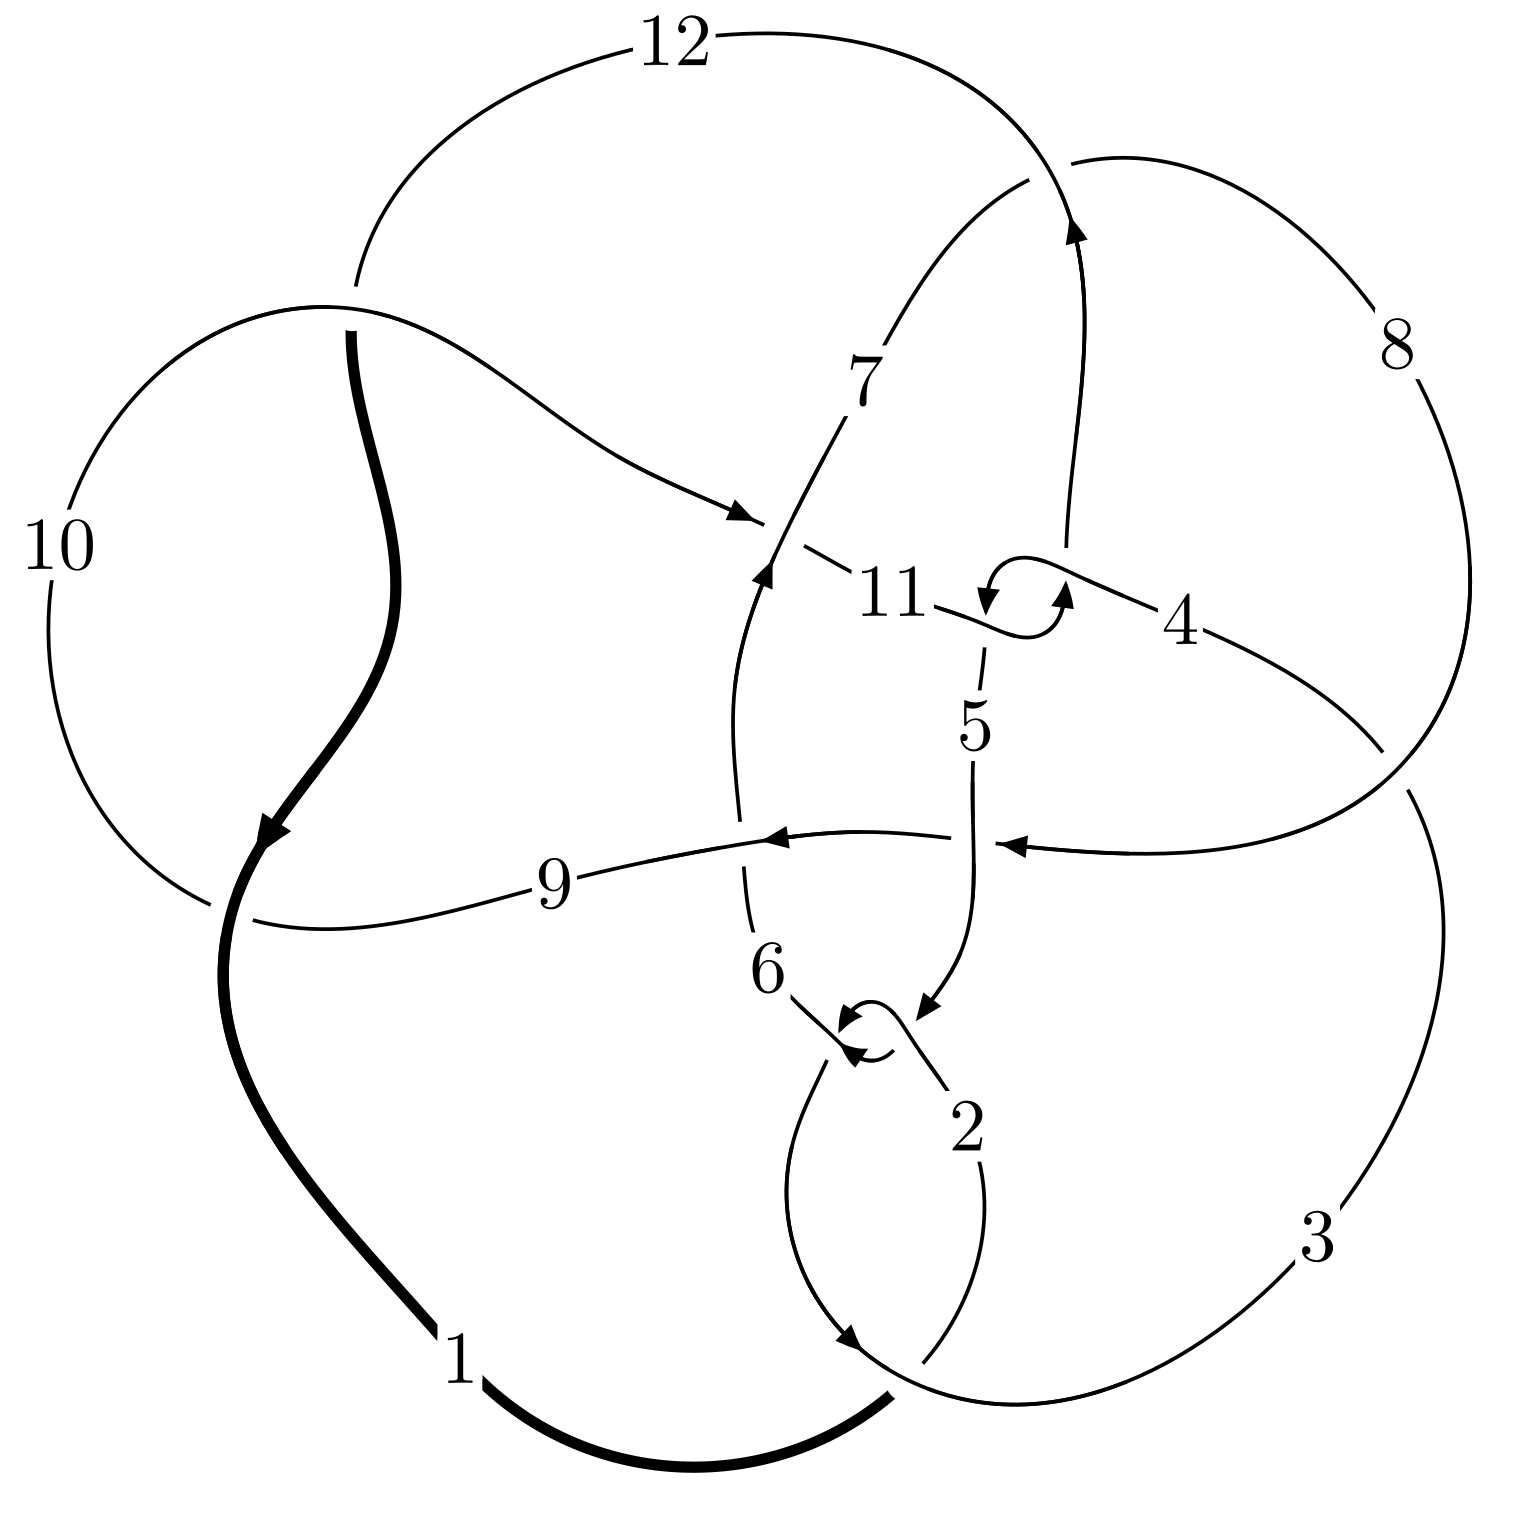
\includegraphics[width=112pt]{../../../GIT/diagram.site/Diagrams/png/1118_12a_0317.png}\\
\ \ \ A knot diagram\footnotemark}&
\allowdisplaybreaks
\textbf{Linearized knot diagam} \\
\cline{2-2}
 &
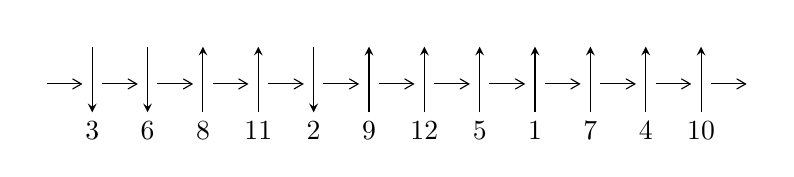
\begin{tikzpicture}[x=20pt, y=17pt]
	% nodes
	\node (C0) at (0, 0) {};
	\node (C1) at (1, 0) {};
	\node (C1U) at (1, +1) {};
	\node (C1D) at (1, -1) {3};

	\node (C2) at (2, 0) {};
	\node (C2U) at (2, +1) {};
	\node (C2D) at (2, -1) {6};

	\node (C3) at (3, 0) {};
	\node (C3U) at (3, +1) {};
	\node (C3D) at (3, -1) {8};

	\node (C4) at (4, 0) {};
	\node (C4U) at (4, +1) {};
	\node (C4D) at (4, -1) {11};

	\node (C5) at (5, 0) {};
	\node (C5U) at (5, +1) {};
	\node (C5D) at (5, -1) {2};

	\node (C6) at (6, 0) {};
	\node (C6U) at (6, +1) {};
	\node (C6D) at (6, -1) {9};

	\node (C7) at (7, 0) {};
	\node (C7U) at (7, +1) {};
	\node (C7D) at (7, -1) {12};

	\node (C8) at (8, 0) {};
	\node (C8U) at (8, +1) {};
	\node (C8D) at (8, -1) {5};

	\node (C9) at (9, 0) {};
	\node (C9U) at (9, +1) {};
	\node (C9D) at (9, -1) {1};

	\node (C10) at (10, 0) {};
	\node (C10U) at (10, +1) {};
	\node (C10D) at (10, -1) {7};

	\node (C11) at (11, 0) {};
	\node (C11U) at (11, +1) {};
	\node (C11D) at (11, -1) {4};

	\node (C12) at (12, 0) {};
	\node (C12U) at (12, +1) {};
	\node (C12D) at (12, -1) {10};
	\node (C13) at (13, 0) {};

	% arrows
	\draw[->,>={angle 60}]
	(C0) edge (C1) (C1) edge (C2) (C2) edge (C3) (C3) edge (C4) (C4) edge (C5) (C5) edge (C6) (C6) edge (C7) (C7) edge (C8) (C8) edge (C9) (C9) edge (C10) (C10) edge (C11) (C11) edge (C12) (C12) edge (C13) ;	\draw[->,>=stealth]
	(C1U) edge (C1D) (C2U) edge (C2D) (C3D) edge (C3U) (C4D) edge (C4U) (C5U) edge (C5D) (C6D) edge (C6U) (C7D) edge (C7U) (C8D) edge (C8U) (C9D) edge (C9U) (C10D) edge (C10U) (C11D) edge (C11U) (C12D) edge (C12U) ;
	\end{tikzpicture} \\
\hhline{~~} \\& 
\textbf{Solving Sequence} \\ \cline{2-2} 
 &
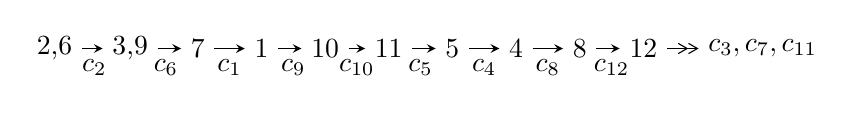
\begin{tikzpicture}[x=23pt, y=7pt]
	% node
	\node (A0) at (-1/8, 0) {2,6};
	\node (A1) at (17/16, 0) {3,9};
	\node (A2) at (17/8, 0) {7};
	\node (A3) at (25/8, 0) {1};
	\node (A4) at (33/8, 0) {10};
	\node (A5) at (41/8, 0) {11};
	\node (A6) at (49/8, 0) {5};
	\node (A7) at (57/8, 0) {4};
	\node (A8) at (65/8, 0) {8};
	\node (A9) at (73/8, 0) {12};
	\node (C1) at (1/2, -1) {$c_{2}$};
	\node (C2) at (13/8, -1) {$c_{6}$};
	\node (C3) at (21/8, -1) {$c_{1}$};
	\node (C4) at (29/8, -1) {$c_{9}$};
	\node (C5) at (37/8, -1) {$c_{10}$};
	\node (C6) at (45/8, -1) {$c_{5}$};
	\node (C7) at (53/8, -1) {$c_{4}$};
	\node (C8) at (61/8, -1) {$c_{8}$};
	\node (C9) at (69/8, -1) {$c_{12}$};
	\node (A10) at (11, 0) {$c_{3},c_{7},c_{11}$};

	% edge
	\draw[->,>=stealth]	
	(A0) edge (A1) (A1) edge (A2) (A2) edge (A3) (A3) edge (A4) (A4) edge (A5) (A5) edge (A6) (A6) edge (A7) (A7) edge (A8) (A8) edge (A9) ;
	\draw[->>,>={angle 60}]	
	(A9) edge (A10);
\end{tikzpicture} \\ 

\end{tabular} \\

\footnotetext{
The image of knot diagram is generated by the software ``\textbf{Draw programme}" developed by Andrew Bartholomew(\url{http://www.layer8.co.uk/maths/draw/index.htm\#Running-draw}), where we modified some parts for our purpose(\url{https://github.com/CATsTAILs/LinksPainter}).
}\phantom \\ \newline 
\centering \textbf{Ideals for irreducible components\footnotemark of $X_{\text{par}}$} 
 
\begin{align*}
I^u_{1}&=\langle 
-2.32563\times10^{433} u^{170}+1.21640\times10^{434} u^{169}+\cdots+1.40890\times10^{433} b-1.01659\times10^{434},\\
\phantom{I^u_{1}}&\phantom{= \langle  }1.54855\times10^{434} u^{170}-5.21699\times10^{434} u^{169}+\cdots+1.40890\times10^{433} a-1.21190\times10^{435},\\
\phantom{I^u_{1}}&\phantom{= \langle  }u^{171}-4 u^{170}+\cdots-15 u+1\rangle \\
I^u_{2}&=\langle 
32195546 u^{41}+78988862 u^{40}+\cdots+764339 b+140677369,\\
\phantom{I^u_{2}}&\phantom{= \langle  }90471926 u^{41}+220915467 u^{40}+\cdots+2293017 a+394515903,\;u^{42}+3 u^{41}+\cdots-26 u^2+3\rangle \\
\\
\end{align*}
\raggedright * 2 irreducible components of $\dim_{\mathbb{C}}=0$, with total 213 representations.\\
\footnotetext{All coefficients of polynomials are rational numbers. But the coefficients are sometimes approximated in decimal forms when there is not enough margin.}
\newpage
\renewcommand{\arraystretch}{1}
\centering \section*{I. $I^u_{1}= \langle -2.33\times10^{433} u^{170}+1.22\times10^{434} u^{169}+\cdots+1.41\times10^{433} b-1.02\times10^{434},\;1.55\times10^{434} u^{170}-5.22\times10^{434} u^{169}+\cdots+1.41\times10^{433} a-1.21\times10^{435},\;u^{171}-4 u^{170}+\cdots-15 u+1 \rangle$}
\flushleft \textbf{(i) Arc colorings}\\
\begin{tabular}{m{7pt} m{180pt} m{7pt} m{180pt} }
\flushright $a_{2}=$&$\begin{pmatrix}1\\0\end{pmatrix}$ \\
\flushright $a_{6}=$&$\begin{pmatrix}0\\u\end{pmatrix}$ \\
\flushright $a_{3}=$&$\begin{pmatrix}1\\u^2\end{pmatrix}$ \\
\flushright $a_{9}=$&$\begin{pmatrix}-10.9912 u^{170}+37.0289 u^{169}+\cdots-657.898 u+86.0181\\1.65068 u^{170}-8.63368 u^{169}+\cdots-35.5431 u+7.21549\end{pmatrix}$ \\
\flushright $a_{7}=$&$\begin{pmatrix}4.08126 u^{170}+16.4331 u^{169}+\cdots-1390.19 u+180.144\\30.3070 u^{170}-84.4218 u^{169}+\cdots+157.355 u-4.90611\end{pmatrix}$ \\
\flushright $a_{1}=$&$\begin{pmatrix}- u^2+1\\- u^4\end{pmatrix}$ \\
\flushright $a_{10}=$&$\begin{pmatrix}-23.2483 u^{170}+71.0398 u^{169}+\cdots-834.056 u+102.538\\-9.46748 u^{170}+18.0078 u^{169}+\cdots-87.8514 u+10.3668\end{pmatrix}$ \\
\flushright $a_{11}=$&$\begin{pmatrix}55.3657 u^{170}-186.121 u^{169}+\cdots+1834.04 u-189.057\\26.3127 u^{170}-71.7091 u^{169}+\cdots+227.304 u-15.1206\end{pmatrix}$ \\
\flushright $a_{5}=$&$\begin{pmatrix}u\\u\end{pmatrix}$ \\
\flushright $a_{4}=$&$\begin{pmatrix}42.9698 u^{170}-160.816 u^{169}+\cdots+1415.01 u-125.166\\15.3205 u^{170}-65.5905 u^{169}+\cdots+387.277 u-26.3923\end{pmatrix}$ \\
\flushright $a_{8}=$&$\begin{pmatrix}-14.8780 u^{170}+50.2409 u^{169}+\cdots-718.830 u+90.9230\\-2.23607 u^{170}+4.57829 u^{169}+\cdots-96.4751 u+12.1204\end{pmatrix}$ \\
\flushright $a_{12}=$&$\begin{pmatrix}8.25459 u^{170}-7.08653 u^{169}+\cdots-609.543 u+67.1361\\35.9201 u^{170}-121.227 u^{169}+\cdots+606.030 u-45.7176\end{pmatrix}$\\&\end{tabular}
\flushleft \textbf{(ii) Obstruction class $= -1$}\\~\\
\flushleft \textbf{(iii) Cusp Shapes $= -73.4828 u^{170}+198.083 u^{169}+\cdots-1119.20 u+108.206$}\\~\\
\newpage\renewcommand{\arraystretch}{1}
\flushleft \textbf{(iv) u-Polynomials at the component}\newline \\
\begin{tabular}{m{50pt}|m{274pt}}
Crossings & \hspace{64pt}u-Polynomials at each crossing \\
\hline $$\begin{aligned}c_{1}\end{aligned}$$&$\begin{aligned}
&u^{171}+82 u^{170}+\cdots+109 u+1
\end{aligned}$\\
\hline $$\begin{aligned}c_{2},c_{5}\end{aligned}$$&$\begin{aligned}
&u^{171}+4 u^{170}+\cdots-15 u-1
\end{aligned}$\\
\hline $$\begin{aligned}c_{3}\end{aligned}$$&$\begin{aligned}
&u^{171}+u^{170}+\cdots+426385251 u-251071867
\end{aligned}$\\
\hline $$\begin{aligned}c_{4},c_{11}\end{aligned}$$&$\begin{aligned}
&u^{171}-2 u^{170}+\cdots+3950 u-1849
\end{aligned}$\\
\hline $$\begin{aligned}c_{6}\end{aligned}$$&$\begin{aligned}
&u^{171}-3 u^{170}+\cdots-148 u-1496
\end{aligned}$\\
\hline $$\begin{aligned}c_{7}\end{aligned}$$&$\begin{aligned}
&u^{171}+2 u^{170}+\cdots-2755517934 u-204636559
\end{aligned}$\\
\hline $$\begin{aligned}c_{8}\end{aligned}$$&$\begin{aligned}
&u^{171}-15 u^{169}+\cdots-541710 u-228281
\end{aligned}$\\
\hline $$\begin{aligned}c_{9},c_{12}\end{aligned}$$&$\begin{aligned}
&u^{171}+11 u^{170}+\cdots-15988 u-3784
\end{aligned}$\\
\hline $$\begin{aligned}c_{10}\end{aligned}$$&$\begin{aligned}
&u^{171}+4 u^{170}+\cdots-974881 u-49723
\end{aligned}$\\
\hline
\end{tabular}\\~\\
\newpage\renewcommand{\arraystretch}{1}
\flushleft \textbf{(v) Riley Polynomials at the component}\newline \\
\begin{tabular}{m{50pt}|m{274pt}}
Crossings & \hspace{64pt}Riley Polynomials at each crossing \\
\hline $$\begin{aligned}c_{1}\end{aligned}$$&$\begin{aligned}
&y^{171}+26 y^{170}+\cdots+2329 y-1
\end{aligned}$\\
\hline $$\begin{aligned}c_{2},c_{5}\end{aligned}$$&$\begin{aligned}
&y^{171}-82 y^{170}+\cdots+109 y-1
\end{aligned}$\\
\hline $$\begin{aligned}c_{3}\end{aligned}$$&$\begin{aligned}
&y^{171}+39 y^{170}+\cdots-1949406148708587857 y-63037082398865689
\end{aligned}$\\
\hline $$\begin{aligned}c_{4},c_{11}\end{aligned}$$&$\begin{aligned}
&y^{171}+106 y^{170}+\cdots-87630868 y-3418801
\end{aligned}$\\
\hline $$\begin{aligned}c_{6}\end{aligned}$$&$\begin{aligned}
&y^{171}+7 y^{170}+\cdots+82092464 y-2238016
\end{aligned}$\\
\hline $$\begin{aligned}c_{7}\end{aligned}$$&$\begin{aligned}
&y^{171}+60 y^{170}+\cdots-3089300280968879260 y-41876121279360481
\end{aligned}$\\
\hline $$\begin{aligned}c_{8}\end{aligned}$$&$\begin{aligned}
&y^{171}-30 y^{170}+\cdots+167534946682 y-52112214961
\end{aligned}$\\
\hline $$\begin{aligned}c_{9},c_{12}\end{aligned}$$&$\begin{aligned}
&y^{171}+131 y^{170}+\cdots-270117680 y-14318656
\end{aligned}$\\
\hline $$\begin{aligned}c_{10}\end{aligned}$$&$\begin{aligned}
&y^{171}+50 y^{170}+\cdots-24962763117 y-2472376729
\end{aligned}$\\
\hline
\end{tabular}\\~\\
\newpage\flushleft \textbf{(vi) Complex Volumes and Cusp Shapes}
$$\begin{array}{c|c|c}  
\text{Solutions to }I^u_{1}& \I (\text{vol} + \sqrt{-1}CS) & \text{Cusp shape}\\
 \hline 
\begin{aligned}
u &= \phantom{-}0.380674 + 0.927822 I \\
a &= -1.44104 + 0.75185 I \\
b &= -0.0853248 - 0.0837685 I\end{aligned}
 & -4.1236 + 14.6388 I & \phantom{-0.000000 } 0 \\ \hline\begin{aligned}
u &= \phantom{-}0.380674 - 0.927822 I \\
a &= -1.44104 - 0.75185 I \\
b &= -0.0853248 + 0.0837685 I\end{aligned}
 & -4.1236 - 14.6388 I & \phantom{-0.000000 } 0 \\ \hline\begin{aligned}
u &= -0.366931 + 0.917472 I \\
a &= \phantom{-}1.24732 + 0.78228 I \\
b &= \phantom{-}0.0952655 + 0.0515088 I\end{aligned}
 & -0.53997 - 8.66240 I & \phantom{-0.000000 } 0 \\ \hline\begin{aligned}
u &= -0.366931 - 0.917472 I \\
a &= \phantom{-}1.24732 - 0.78228 I \\
b &= \phantom{-}0.0952655 - 0.0515088 I\end{aligned}
 & -0.53997 + 8.66240 I & \phantom{-0.000000 } 0 \\ \hline\begin{aligned}
u &= \phantom{-}0.342928 + 0.920390 I \\
a &= -1.043760 + 0.494653 I \\
b &= \phantom{-}0.066645 + 0.176467 I\end{aligned}
 & -6.04580 + 3.49754 I & \phantom{-0.000000 } 0 \\ \hline\begin{aligned}
u &= \phantom{-}0.342928 - 0.920390 I \\
a &= -1.043760 - 0.494653 I \\
b &= \phantom{-}0.066645 - 0.176467 I\end{aligned}
 & -6.04580 - 3.49754 I & \phantom{-0.000000 } 0 \\ \hline\begin{aligned}
u &= -0.457582 + 0.853117 I \\
a &= \phantom{-}0.495659 + 0.753146 I \\
b &= \phantom{-}0.062593 + 0.311303 I\end{aligned}
 & \phantom{-}3.31452 - 0.97599 I & \phantom{-0.000000 } 0 \\ \hline\begin{aligned}
u &= -0.457582 - 0.853117 I \\
a &= \phantom{-}0.495659 - 0.753146 I \\
b &= \phantom{-}0.062593 - 0.311303 I\end{aligned}
 & \phantom{-}3.31452 + 0.97599 I & \phantom{-0.000000 } 0 \\ \hline\begin{aligned}
u &= \phantom{-}0.513246 + 0.819161 I \\
a &= -0.400049 + 1.051320 I \\
b &= -0.250673 + 0.288197 I\end{aligned}
 & \phantom{-}0.55062 - 5.32202 I & \phantom{-0.000000 } 0 \\ \hline\begin{aligned}
u &= \phantom{-}0.513246 - 0.819161 I \\
a &= -0.400049 - 1.051320 I \\
b &= -0.250673 - 0.288197 I\end{aligned}
 & \phantom{-}0.55062 + 5.32202 I & \phantom{-0.000000 } 0\\
 \hline 
 \end{array}$$\newpage$$\begin{array}{c|c|c}  
\text{Solutions to }I^u_{1}& \I (\text{vol} + \sqrt{-1}CS) & \text{Cusp shape}\\
 \hline 
\begin{aligned}
u &= -0.963158 + 0.402921 I \\
a &= -0.200696 - 0.192810 I \\
b &= \phantom{-}1.95696 - 1.21862 I\end{aligned}
 & -6.54806 - 0.36272 I & \phantom{-0.000000 } 0 \\ \hline\begin{aligned}
u &= -0.963158 - 0.402921 I \\
a &= -0.200696 + 0.192810 I \\
b &= \phantom{-}1.95696 + 1.21862 I\end{aligned}
 & -6.54806 + 0.36272 I & \phantom{-0.000000 } 0 \\ \hline\begin{aligned}
u &= -0.902678 + 0.300350 I \\
a &= \phantom{-}0.169921 - 0.476034 I \\
b &= \phantom{-}0.31990 - 2.60195 I\end{aligned}
 & -6.00184 + 3.22017 I & \phantom{-0.000000 } 0 \\ \hline\begin{aligned}
u &= -0.902678 - 0.300350 I \\
a &= \phantom{-}0.169921 + 0.476034 I \\
b &= \phantom{-}0.31990 + 2.60195 I\end{aligned}
 & -6.00184 - 3.22017 I & \phantom{-0.000000 } 0 \\ \hline\begin{aligned}
u &= -0.524370 + 0.789822 I \\
a &= \phantom{-}0.952807 + 0.482256 I \\
b &= -0.327914 - 0.000260 I\end{aligned}
 & \phantom{-}3.81793 - 2.46825 I & \phantom{-0.000000 } 0 \\ \hline\begin{aligned}
u &= -0.524370 - 0.789822 I \\
a &= \phantom{-}0.952807 - 0.482256 I \\
b &= -0.327914 + 0.000260 I\end{aligned}
 & \phantom{-}3.81793 + 2.46825 I & \phantom{-0.000000 } 0 \\ \hline\begin{aligned}
u &= \phantom{-}0.619006 + 0.717514 I \\
a &= \phantom{-}1.45978 - 0.38331 I \\
b &= \phantom{-}0.984183 - 0.260417 I\end{aligned}
 & -0.55947 + 2.06152 I & \phantom{-0.000000 } 0 \\ \hline\begin{aligned}
u &= \phantom{-}0.619006 - 0.717514 I \\
a &= \phantom{-}1.45978 + 0.38331 I \\
b &= \phantom{-}0.984183 + 0.260417 I\end{aligned}
 & -0.55947 - 2.06152 I & \phantom{-0.000000 } 0 \\ \hline\begin{aligned}
u &= -0.963099 + 0.428193 I \\
a &= -1.078290 + 0.719454 I \\
b &= \phantom{-}0.04140 + 1.50915 I\end{aligned}
 & -4.11245 - 0.56172 I & \phantom{-0.000000 } 0 \\ \hline\begin{aligned}
u &= -0.963099 - 0.428193 I \\
a &= -1.078290 - 0.719454 I \\
b &= \phantom{-}0.04140 - 1.50915 I\end{aligned}
 & -4.11245 + 0.56172 I & \phantom{-0.000000 } 0\\
 \hline 
 \end{array}$$\newpage$$\begin{array}{c|c|c}  
\text{Solutions to }I^u_{1}& \I (\text{vol} + \sqrt{-1}CS) & \text{Cusp shape}\\
 \hline 
\begin{aligned}
u &= \phantom{-}0.983442 + 0.380664 I \\
a &= -0.088813 + 0.216542 I \\
b &= \phantom{-}0.422686 + 0.496267 I\end{aligned}
 & -1.69986 - 1.28381 I & \phantom{-0.000000 } 0 \\ \hline\begin{aligned}
u &= \phantom{-}0.983442 - 0.380664 I \\
a &= -0.088813 - 0.216542 I \\
b &= \phantom{-}0.422686 - 0.496267 I\end{aligned}
 & -1.69986 + 1.28381 I & \phantom{-0.000000 } 0 \\ \hline\begin{aligned}
u &= -0.608840 + 0.864426 I \\
a &= -1.46352 - 0.29358 I \\
b &= -0.760839 + 0.330719 I\end{aligned}
 & -0.89924 - 4.15334 I & \phantom{-0.000000 } 0 \\ \hline\begin{aligned}
u &= -0.608840 - 0.864426 I \\
a &= -1.46352 + 0.29358 I \\
b &= -0.760839 - 0.330719 I\end{aligned}
 & -0.89924 + 4.15334 I & \phantom{-0.000000 } 0 \\ \hline\begin{aligned}
u &= -0.852708 + 0.633407 I \\
a &= -0.067536 + 0.409120 I \\
b &= \phantom{-}0.288912 + 1.118510 I\end{aligned}
 & \phantom{-}1.80657 + 0.58573 I & \phantom{-0.000000 } 0 \\ \hline\begin{aligned}
u &= -0.852708 - 0.633407 I \\
a &= -0.067536 - 0.409120 I \\
b &= \phantom{-}0.288912 - 1.118510 I\end{aligned}
 & \phantom{-}1.80657 - 0.58573 I & \phantom{-0.000000 } 0 \\ \hline\begin{aligned}
u &= \phantom{-}0.601646 + 0.717900 I \\
a &= \phantom{-}0.722399 + 0.676708 I \\
b &= -0.061865 + 0.750125 I\end{aligned}
 & -1.72699 + 3.31478 I & \phantom{-0.000000 } 0 \\ \hline\begin{aligned}
u &= \phantom{-}0.601646 - 0.717900 I \\
a &= \phantom{-}0.722399 - 0.676708 I \\
b &= -0.061865 - 0.750125 I\end{aligned}
 & -1.72699 - 3.31478 I & \phantom{-0.000000 } 0 \\ \hline\begin{aligned}
u &= \phantom{-}0.472074 + 0.807039 I \\
a &= -1.224110 + 0.555132 I \\
b &= \phantom{-}0.324520 - 0.201902 I\end{aligned}
 & \phantom{-}0.35785 + 8.72561 I & \phantom{-0.000000 } 0 \\ \hline\begin{aligned}
u &= \phantom{-}0.472074 - 0.807039 I \\
a &= -1.224110 - 0.555132 I \\
b &= \phantom{-}0.324520 + 0.201902 I\end{aligned}
 & \phantom{-}0.35785 - 8.72561 I & \phantom{-0.000000 } 0\\
 \hline 
 \end{array}$$\newpage$$\begin{array}{c|c|c}  
\text{Solutions to }I^u_{1}& \I (\text{vol} + \sqrt{-1}CS) & \text{Cusp shape}\\
 \hline 
\begin{aligned}
u &= \phantom{-}0.910458 + 0.553549 I \\
a &= \phantom{-}0.609592 - 1.005530 I \\
b &= \phantom{-}0.59333 - 1.73565 I\end{aligned}
 & \phantom{-}2.17789 - 2.71349 I & \phantom{-0.000000 } 0 \\ \hline\begin{aligned}
u &= \phantom{-}0.910458 - 0.553549 I \\
a &= \phantom{-}0.609592 + 1.005530 I \\
b &= \phantom{-}0.59333 + 1.73565 I\end{aligned}
 & \phantom{-}2.17789 + 2.71349 I & \phantom{-0.000000 } 0 \\ \hline\begin{aligned}
u &= \phantom{-}0.737359 + 0.574044 I \\
a &= \phantom{-}1.24787 - 0.67806 I \\
b &= \phantom{-}0.387336 - 0.505592 I\end{aligned}
 & \phantom{-}2.70711 - 1.80349 I & \phantom{-0.000000 } 0 \\ \hline\begin{aligned}
u &= \phantom{-}0.737359 - 0.574044 I \\
a &= \phantom{-}1.24787 + 0.67806 I \\
b &= \phantom{-}0.387336 + 0.505592 I\end{aligned}
 & \phantom{-}2.70711 + 1.80349 I & \phantom{-0.000000 } 0 \\ \hline\begin{aligned}
u &= -0.996064 + 0.412530 I \\
a &= \phantom{-}1.23619 - 1.36760 I \\
b &= \phantom{-}0.83346 - 1.99349 I\end{aligned}
 & -4.94892 + 4.79852 I & \phantom{-0.000000 } 0 \\ \hline\begin{aligned}
u &= -0.996064 - 0.412530 I \\
a &= \phantom{-}1.23619 + 1.36760 I \\
b &= \phantom{-}0.83346 + 1.99349 I\end{aligned}
 & -4.94892 - 4.79852 I & \phantom{-0.000000 } 0 \\ \hline\begin{aligned}
u &= -1.027420 + 0.328668 I \\
a &= -0.534851 + 0.323176 I \\
b &= -1.63930 + 1.42441 I\end{aligned}
 & -1.98076 + 0.78863 I & \phantom{-0.000000 } 0 \\ \hline\begin{aligned}
u &= -1.027420 - 0.328668 I \\
a &= -0.534851 - 0.323176 I \\
b &= -1.63930 - 1.42441 I\end{aligned}
 & -1.98076 - 0.78863 I & \phantom{-0.000000 } 0 \\ \hline\begin{aligned}
u &= -0.652142 + 0.649935 I \\
a &= -1.54760 - 0.45381 I \\
b &= -0.480196 + 0.209602 I\end{aligned}
 & \phantom{-}2.49581 - 1.32359 I & \phantom{-0.000000 } 0 \\ \hline\begin{aligned}
u &= -0.652142 - 0.649935 I \\
a &= -1.54760 + 0.45381 I \\
b &= -0.480196 - 0.209602 I\end{aligned}
 & \phantom{-}2.49581 + 1.32359 I & \phantom{-0.000000 } 0\\
 \hline 
 \end{array}$$\newpage$$\begin{array}{c|c|c}  
\text{Solutions to }I^u_{1}& \I (\text{vol} + \sqrt{-1}CS) & \text{Cusp shape}\\
 \hline 
\begin{aligned}
u &= -0.906002 + 0.159736 I \\
a &= \phantom{-}0.689025 + 0.974067 I \\
b &= -0.03277 + 2.18678 I\end{aligned}
 & -6.22172 - 2.61465 I & \phantom{-0.000000 } 0 \\ \hline\begin{aligned}
u &= -0.906002 - 0.159736 I \\
a &= \phantom{-}0.689025 - 0.974067 I \\
b &= -0.03277 - 2.18678 I\end{aligned}
 & -6.22172 + 2.61465 I & \phantom{-0.000000 } 0 \\ \hline\begin{aligned}
u &= -0.869676 + 0.299010 I \\
a &= -1.04273 + 1.82876 I \\
b &= -0.67765 + 2.07453 I\end{aligned}
 & -4.15612 - 1.96479 I & \phantom{-0.000000 } 0 \\ \hline\begin{aligned}
u &= -0.869676 - 0.299010 I \\
a &= -1.04273 - 1.82876 I \\
b &= -0.67765 - 2.07453 I\end{aligned}
 & -4.15612 + 1.96479 I & \phantom{-0.000000 } 0 \\ \hline\begin{aligned}
u &= -1.064860 + 0.185668 I \\
a &= -0.629574 + 1.258680 I \\
b &= -1.21135 + 2.25302 I\end{aligned}
 & -5.13287 - 3.61597 I & \phantom{-0.000000 } 0 \\ \hline\begin{aligned}
u &= -1.064860 - 0.185668 I \\
a &= -0.629574 - 1.258680 I \\
b &= -1.21135 - 2.25302 I\end{aligned}
 & -5.13287 + 3.61597 I & \phantom{-0.000000 } 0 \\ \hline\begin{aligned}
u &= \phantom{-}1.077930 + 0.132381 I \\
a &= -0.464354 + 0.339009 I \\
b &= -0.465901 + 1.022110 I\end{aligned}
 & -2.06028 - 1.44412 I & \phantom{-0.000000 } 0 \\ \hline\begin{aligned}
u &= \phantom{-}1.077930 - 0.132381 I \\
a &= -0.464354 - 0.339009 I \\
b &= -0.465901 - 1.022110 I\end{aligned}
 & -2.06028 + 1.44412 I & \phantom{-0.000000 } 0 \\ \hline\begin{aligned}
u &= -0.770478 + 0.767055 I \\
a &= \phantom{-}0.407056 + 0.408084 I \\
b &= -0.218278 - 0.150888 I\end{aligned}
 & \phantom{-}2.06081 + 4.74559 I & \phantom{-0.000000 } 0 \\ \hline\begin{aligned}
u &= -0.770478 - 0.767055 I \\
a &= \phantom{-}0.407056 - 0.408084 I \\
b &= -0.218278 + 0.150888 I\end{aligned}
 & \phantom{-}2.06081 - 4.74559 I & \phantom{-0.000000 } 0\\
 \hline 
 \end{array}$$\newpage$$\begin{array}{c|c|c}  
\text{Solutions to }I^u_{1}& \I (\text{vol} + \sqrt{-1}CS) & \text{Cusp shape}\\
 \hline 
\begin{aligned}
u &= \phantom{-}0.993773 + 0.458962 I \\
a &= -1.99976 - 1.52669 I \\
b &= -1.85743 - 2.32894 I\end{aligned}
 & -7.53815 - 8.95364 I & \phantom{-0.000000 } 0 \\ \hline\begin{aligned}
u &= \phantom{-}0.993773 - 0.458962 I \\
a &= -1.99976 + 1.52669 I \\
b &= -1.85743 + 2.32894 I\end{aligned}
 & -7.53815 + 8.95364 I & \phantom{-0.000000 } 0 \\ \hline\begin{aligned}
u &= -0.832496 + 0.341495 I \\
a &= \phantom{-}0.22368 - 1.39703 I \\
b &= -0.68750 - 2.12663 I\end{aligned}
 & -3.47452 + 3.78054 I & \phantom{-0.000000 } 0 \\ \hline\begin{aligned}
u &= -0.832496 - 0.341495 I \\
a &= \phantom{-}0.22368 + 1.39703 I \\
b &= -0.68750 + 2.12663 I\end{aligned}
 & -3.47452 - 3.78054 I & \phantom{-0.000000 } 0 \\ \hline\begin{aligned}
u &= -1.004720 + 0.455046 I \\
a &= \phantom{-}0.95877 + 1.80347 I \\
b &= \phantom{-}0.13848 + 2.70177 I\end{aligned}
 & -7.53406 - 3.01774 I & \phantom{-0.000000 } 0 \\ \hline\begin{aligned}
u &= -1.004720 - 0.455046 I \\
a &= \phantom{-}0.95877 - 1.80347 I \\
b &= \phantom{-}0.13848 - 2.70177 I\end{aligned}
 & -7.53406 + 3.01774 I & \phantom{-0.000000 } 0 \\ \hline\begin{aligned}
u &= \phantom{-}0.997250 + 0.488051 I \\
a &= \phantom{-}0.503407 - 0.672180 I \\
b &= -0.87705 - 1.19948 I\end{aligned}
 & -3.62922 - 6.25773 I & \phantom{-0.000000 } 0 \\ \hline\begin{aligned}
u &= \phantom{-}0.997250 - 0.488051 I \\
a &= \phantom{-}0.503407 + 0.672180 I \\
b &= -0.87705 + 1.19948 I\end{aligned}
 & -3.62922 + 6.25773 I & \phantom{-0.000000 } 0 \\ \hline\begin{aligned}
u &= \phantom{-}0.877140 + 0.148952 I \\
a &= \phantom{-}0.319254 - 0.244380 I \\
b &= \phantom{-}1.383800 - 0.021803 I\end{aligned}
 & -1.94154 - 1.69217 I & \phantom{-0.000000 } 0 \\ \hline\begin{aligned}
u &= \phantom{-}0.877140 - 0.148952 I \\
a &= \phantom{-}0.319254 + 0.244380 I \\
b &= \phantom{-}1.383800 + 0.021803 I\end{aligned}
 & -1.94154 + 1.69217 I & \phantom{-0.000000 } 0\\
 \hline 
 \end{array}$$\newpage$$\begin{array}{c|c|c}  
\text{Solutions to }I^u_{1}& \I (\text{vol} + \sqrt{-1}CS) & \text{Cusp shape}\\
 \hline 
\begin{aligned}
u &= -0.551191 + 0.697646 I \\
a &= -0.718557 - 0.424698 I \\
b &= -0.000171 + 0.443670 I\end{aligned}
 & \phantom{-}1.83304 - 0.04257 I & \phantom{-0.000000 } 0 \\ \hline\begin{aligned}
u &= -0.551191 - 0.697646 I \\
a &= -0.718557 + 0.424698 I \\
b &= -0.000171 - 0.443670 I\end{aligned}
 & \phantom{-}1.83304 + 0.04257 I & \phantom{-0.000000 } 0 \\ \hline\begin{aligned}
u &= -1.113720 + 0.007895 I \\
a &= \phantom{-}0.696014 - 0.362883 I \\
b &= \phantom{-}1.28502 - 1.37620 I\end{aligned}
 & -5.25534 - 6.96011 I & \phantom{-0.000000 } 0 \\ \hline\begin{aligned}
u &= -1.113720 - 0.007895 I \\
a &= \phantom{-}0.696014 + 0.362883 I \\
b &= \phantom{-}1.28502 + 1.37620 I\end{aligned}
 & -5.25534 + 6.96011 I & \phantom{-0.000000 } 0 \\ \hline\begin{aligned}
u &= -0.397409 + 0.784388 I \\
a &= -1.61735 - 0.84389 I \\
b &= -0.346025 - 0.010243 I\end{aligned}
 & \phantom{-}0.88603 - 2.61590 I & \phantom{-0.000000 } 0 \\ \hline\begin{aligned}
u &= -0.397409 - 0.784388 I \\
a &= -1.61735 + 0.84389 I \\
b &= -0.346025 + 0.010243 I\end{aligned}
 & \phantom{-}0.88603 + 2.61590 I & \phantom{-0.000000 } 0 \\ \hline\begin{aligned}
u &= \phantom{-}1.001020 + 0.506622 I \\
a &= \phantom{-}0.362424 + 0.558521 I \\
b &= -1.11134 + 2.02291 I\end{aligned}
 & -5.78670 - 6.09009 I & \phantom{-0.000000 } 0 \\ \hline\begin{aligned}
u &= \phantom{-}1.001020 - 0.506622 I \\
a &= \phantom{-}0.362424 - 0.558521 I \\
b &= -1.11134 - 2.02291 I\end{aligned}
 & -5.78670 + 6.09009 I & \phantom{-0.000000 } 0 \\ \hline\begin{aligned}
u &= -0.070999 + 0.872170 I \\
a &= \phantom{-}0.222455 - 0.293730 I \\
b &= -0.079710 + 0.800694 I\end{aligned}
 & -4.04271 + 0.14105 I & \phantom{-0.000000 } 0 \\ \hline\begin{aligned}
u &= -0.070999 - 0.872170 I \\
a &= \phantom{-}0.222455 + 0.293730 I \\
b &= -0.079710 - 0.800694 I\end{aligned}
 & -4.04271 - 0.14105 I & \phantom{-0.000000 } 0\\
 \hline 
 \end{array}$$\newpage$$\begin{array}{c|c|c}  
\text{Solutions to }I^u_{1}& \I (\text{vol} + \sqrt{-1}CS) & \text{Cusp shape}\\
 \hline 
\begin{aligned}
u &= \phantom{-}1.062620 + 0.373348 I \\
a &= \phantom{-}0.669379 + 1.159990 I \\
b &= -0.00720 + 2.58624 I\end{aligned}
 & -9.42963 + 3.52313 I & \phantom{-0.000000 } 0 \\ \hline\begin{aligned}
u &= \phantom{-}1.062620 - 0.373348 I \\
a &= \phantom{-}0.669379 - 1.159990 I \\
b &= -0.00720 - 2.58624 I\end{aligned}
 & -9.42963 - 3.52313 I & \phantom{-0.000000 } 0 \\ \hline\begin{aligned}
u &= \phantom{-}1.029440 + 0.468018 I \\
a &= -0.679986 + 1.187760 I \\
b &= \phantom{-}0.03796 + 1.87433 I\end{aligned}
 & -4.50899 - 1.41426 I & \phantom{-0.000000 } 0 \\ \hline\begin{aligned}
u &= \phantom{-}1.029440 - 0.468018 I \\
a &= -0.679986 - 1.187760 I \\
b &= \phantom{-}0.03796 - 1.87433 I\end{aligned}
 & -4.50899 + 1.41426 I & \phantom{-0.000000 } 0 \\ \hline\begin{aligned}
u &= -1.055360 + 0.416777 I \\
a &= \phantom{-}1.41093 + 0.56066 I \\
b &= \phantom{-}1.10806 + 1.28031 I\end{aligned}
 & -7.87632 + 5.00657 I & \phantom{-0.000000 } 0 \\ \hline\begin{aligned}
u &= -1.055360 - 0.416777 I \\
a &= \phantom{-}1.41093 - 0.56066 I \\
b &= \phantom{-}1.10806 - 1.28031 I\end{aligned}
 & -7.87632 - 5.00657 I & \phantom{-0.000000 } 0 \\ \hline\begin{aligned}
u &= \phantom{-}1.128130 + 0.138441 I \\
a &= \phantom{-}0.490406 + 1.029600 I \\
b &= \phantom{-}1.21506 + 1.53210 I\end{aligned}
 & -4.14419 + 0.26617 I & \phantom{-0.000000 } 0 \\ \hline\begin{aligned}
u &= \phantom{-}1.128130 - 0.138441 I \\
a &= \phantom{-}0.490406 - 1.029600 I \\
b &= \phantom{-}1.21506 - 1.53210 I\end{aligned}
 & -4.14419 - 0.26617 I & \phantom{-0.000000 } 0 \\ \hline\begin{aligned}
u &= -0.974222 + 0.606012 I \\
a &= -0.362252 - 1.303630 I \\
b &= -0.89790 - 2.06897 I\end{aligned}
 & \phantom{-}1.51676 + 6.24193 I & \phantom{-0.000000 } 0 \\ \hline\begin{aligned}
u &= -0.974222 - 0.606012 I \\
a &= -0.362252 + 1.303630 I \\
b &= -0.89790 + 2.06897 I\end{aligned}
 & \phantom{-}1.51676 - 6.24193 I & \phantom{-0.000000 } 0\\
 \hline 
 \end{array}$$\newpage$$\begin{array}{c|c|c}  
\text{Solutions to }I^u_{1}& \I (\text{vol} + \sqrt{-1}CS) & \text{Cusp shape}\\
 \hline 
\begin{aligned}
u &= \phantom{-}0.411540 + 0.737500 I \\
a &= \phantom{-}1.98145 - 0.41932 I \\
b &= \phantom{-}0.198004 - 0.081694 I\end{aligned}
 & -0.52582 + 5.71309 I & \phantom{-0.000000 } 0 \\ \hline\begin{aligned}
u &= \phantom{-}0.411540 - 0.737500 I \\
a &= \phantom{-}1.98145 + 0.41932 I \\
b &= \phantom{-}0.198004 + 0.081694 I\end{aligned}
 & -0.52582 - 5.71309 I & \phantom{-0.000000 } 0 \\ \hline\begin{aligned}
u &= \phantom{-}1.041990 + 0.524020 I \\
a &= \phantom{-}0.188332 + 0.059206 I \\
b &= \phantom{-}0.858931 + 0.001148 I\end{aligned}
 & -1.60249 - 1.20863 I & \phantom{-0.000000 } 0 \\ \hline\begin{aligned}
u &= \phantom{-}1.041990 - 0.524020 I \\
a &= \phantom{-}0.188332 - 0.059206 I \\
b &= \phantom{-}0.858931 - 0.001148 I\end{aligned}
 & -1.60249 + 1.20863 I & \phantom{-0.000000 } 0 \\ \hline\begin{aligned}
u &= \phantom{-}0.504932 + 0.663071 I \\
a &= -0.029547 - 1.046380 I \\
b &= -0.144795 + 0.279639 I\end{aligned}
 & -0.01068 - 3.46818 I & \phantom{-0.000000 } 0 \\ \hline\begin{aligned}
u &= \phantom{-}0.504932 - 0.663071 I \\
a &= -0.029547 + 1.046380 I \\
b &= -0.144795 - 0.279639 I\end{aligned}
 & -0.01068 + 3.46818 I & \phantom{-0.000000 } 0 \\ \hline\begin{aligned}
u &= \phantom{-}1.030840 + 0.550584 I \\
a &= \phantom{-}0.081680 + 0.737119 I \\
b &= \phantom{-}0.07377 + 2.27695 I\end{aligned}
 & -4.12716 - 2.65231 I & \phantom{-0.000000 } 0 \\ \hline\begin{aligned}
u &= \phantom{-}1.030840 - 0.550584 I \\
a &= \phantom{-}0.081680 - 0.737119 I \\
b &= \phantom{-}0.07377 - 2.27695 I\end{aligned}
 & -4.12716 + 2.65231 I & \phantom{-0.000000 } 0 \\ \hline\begin{aligned}
u &= \phantom{-}1.077090 + 0.455377 I \\
a &= -1.59679 - 0.24739 I \\
b &= -1.63729 - 0.38978 I\end{aligned}
 & -7.57854 - 1.92005 I & \phantom{-0.000000 } 0 \\ \hline\begin{aligned}
u &= \phantom{-}1.077090 - 0.455377 I \\
a &= -1.59679 + 0.24739 I \\
b &= -1.63729 + 0.38978 I\end{aligned}
 & -7.57854 + 1.92005 I & \phantom{-0.000000 } 0\\
 \hline 
 \end{array}$$\newpage$$\begin{array}{c|c|c}  
\text{Solutions to }I^u_{1}& \I (\text{vol} + \sqrt{-1}CS) & \text{Cusp shape}\\
 \hline 
\begin{aligned}
u &= -1.065590 + 0.482857 I \\
a &= -0.032303 - 0.881627 I \\
b &= \phantom{-}1.24334 - 2.14322 I\end{aligned}
 & -8.70093 + 10.41120 I & \phantom{-0.000000 } 0 \\ \hline\begin{aligned}
u &= -1.065590 - 0.482857 I \\
a &= -0.032303 + 0.881627 I \\
b &= \phantom{-}1.24334 + 2.14322 I\end{aligned}
 & -8.70093 - 10.41120 I & \phantom{-0.000000 } 0 \\ \hline\begin{aligned}
u &= \phantom{-}0.447936 + 1.084730 I \\
a &= \phantom{-}0.793300 - 0.275904 I \\
b &= \phantom{-}0.106561 + 0.242441 I\end{aligned}
 & -4.09201 + 3.51596 I & \phantom{-0.000000 } 0 \\ \hline\begin{aligned}
u &= \phantom{-}0.447936 - 1.084730 I \\
a &= \phantom{-}0.793300 + 0.275904 I \\
b &= \phantom{-}0.106561 - 0.242441 I\end{aligned}
 & -4.09201 - 3.51596 I & \phantom{-0.000000 } 0 \\ \hline\begin{aligned}
u &= \phantom{-}0.774135 + 0.887136 I \\
a &= -0.285418 + 0.534779 I \\
b &= -0.025746 - 0.229887 I\end{aligned}
 & -1.76625 - 10.05830 I & \phantom{-0.000000 } 0 \\ \hline\begin{aligned}
u &= \phantom{-}0.774135 - 0.887136 I \\
a &= -0.285418 - 0.534779 I \\
b &= -0.025746 + 0.229887 I\end{aligned}
 & -1.76625 + 10.05830 I & \phantom{-0.000000 } 0 \\ \hline\begin{aligned}
u &= \phantom{-}1.057200 + 0.522195 I \\
a &= \phantom{-}0.319475 - 1.147410 I \\
b &= \phantom{-}1.15222 - 2.70949 I\end{aligned}
 & -0.68694 - 5.83662 I & \phantom{-0.000000 } 0 \\ \hline\begin{aligned}
u &= \phantom{-}1.057200 - 0.522195 I \\
a &= \phantom{-}0.319475 + 1.147410 I \\
b &= \phantom{-}1.15222 + 2.70949 I\end{aligned}
 & -0.68694 + 5.83662 I & \phantom{-0.000000 } 0 \\ \hline\begin{aligned}
u &= \phantom{-}1.014160 + 0.611681 I \\
a &= \phantom{-}0.49863 - 1.52419 I \\
b &= \phantom{-}0.42736 - 1.97683 I\end{aligned}
 & -1.77729 - 7.16397 I & \phantom{-0.000000 } 0 \\ \hline\begin{aligned}
u &= \phantom{-}1.014160 - 0.611681 I \\
a &= \phantom{-}0.49863 + 1.52419 I \\
b &= \phantom{-}0.42736 + 1.97683 I\end{aligned}
 & -1.77729 + 7.16397 I & \phantom{-0.000000 } 0\\
 \hline 
 \end{array}$$\newpage$$\begin{array}{c|c|c}  
\text{Solutions to }I^u_{1}& \I (\text{vol} + \sqrt{-1}CS) & \text{Cusp shape}\\
 \hline 
\begin{aligned}
u &= -0.490276 + 0.649949 I \\
a &= -1.25407 - 0.97607 I \\
b &= \phantom{-}0.044037 + 0.412853 I\end{aligned}
 & \phantom{-}2.05585 + 0.51972 I & \phantom{-0.000000 } 0 \\ \hline\begin{aligned}
u &= -0.490276 - 0.649949 I \\
a &= -1.25407 + 0.97607 I \\
b &= \phantom{-}0.044037 - 0.412853 I\end{aligned}
 & \phantom{-}2.05585 - 0.51972 I & \phantom{-0.000000 } 0 \\ \hline\begin{aligned}
u &= -1.046380 + 0.570637 I \\
a &= -0.472941 - 0.969669 I \\
b &= -1.49813 - 1.94744 I\end{aligned}
 & \phantom{-}0.42171 + 4.26907 I & \phantom{-0.000000 } 0 \\ \hline\begin{aligned}
u &= -1.046380 - 0.570637 I \\
a &= -0.472941 + 0.969669 I \\
b &= -1.49813 + 1.94744 I\end{aligned}
 & \phantom{-}0.42171 - 4.26907 I & \phantom{-0.000000 } 0 \\ \hline\begin{aligned}
u &= -1.042350 + 0.593238 I \\
a &= -0.023763 - 0.780552 I \\
b &= -0.60275 - 1.50249 I\end{aligned}
 & \phantom{-}0.34557 + 5.01997 I & \phantom{-0.000000 } 0 \\ \hline\begin{aligned}
u &= -1.042350 - 0.593238 I \\
a &= -0.023763 + 0.780552 I \\
b &= -0.60275 + 1.50249 I\end{aligned}
 & \phantom{-}0.34557 - 5.01997 I & \phantom{-0.000000 } 0 \\ \hline\begin{aligned}
u &= -0.201828 + 0.771335 I \\
a &= -0.90135 - 1.61437 I \\
b &= -0.191801 - 0.131891 I\end{aligned}
 & \phantom{-}1.10724 - 2.01592 I & \phantom{-0.000000 } 0 \\ \hline\begin{aligned}
u &= -0.201828 - 0.771335 I \\
a &= -0.90135 + 1.61437 I \\
b &= -0.191801 + 0.131891 I\end{aligned}
 & \phantom{-}1.10724 + 2.01592 I & \phantom{-0.000000 } 0 \\ \hline\begin{aligned}
u &= \phantom{-}1.167640 + 0.293720 I \\
a &= -0.192728 - 0.745197 I \\
b &= \phantom{-}0.783957 - 1.173730 I\end{aligned}
 & -8.30514 - 3.98448 I & \phantom{-0.000000 } 0 \\ \hline\begin{aligned}
u &= \phantom{-}1.167640 - 0.293720 I \\
a &= -0.192728 + 0.745197 I \\
b &= \phantom{-}0.783957 + 1.173730 I\end{aligned}
 & -8.30514 + 3.98448 I & \phantom{-0.000000 } 0\\
 \hline 
 \end{array}$$\newpage$$\begin{array}{c|c|c}  
\text{Solutions to }I^u_{1}& \I (\text{vol} + \sqrt{-1}CS) & \text{Cusp shape}\\
 \hline 
\begin{aligned}
u &= \phantom{-}1.045390 + 0.627865 I \\
a &= -0.549568 - 0.896469 I \\
b &= -0.26589 - 1.78659 I\end{aligned}
 & -3.10720 - 8.54200 I & \phantom{-0.000000 } 0 \\ \hline\begin{aligned}
u &= \phantom{-}1.045390 - 0.627865 I \\
a &= -0.549568 + 0.896469 I \\
b &= -0.26589 + 1.78659 I\end{aligned}
 & -3.10720 + 8.54200 I & \phantom{-0.000000 } 0 \\ \hline\begin{aligned}
u &= \phantom{-}0.709475 + 0.317529 I \\
a &= \phantom{-}0.70726 + 2.86628 I \\
b &= \phantom{-}0.40349 + 2.30893 I\end{aligned}
 & -6.41519 + 5.46475 I & \phantom{-0.000000 } 0 \\ \hline\begin{aligned}
u &= \phantom{-}0.709475 - 0.317529 I \\
a &= \phantom{-}0.70726 - 2.86628 I \\
b &= \phantom{-}0.40349 - 2.30893 I\end{aligned}
 & -6.41519 - 5.46475 I & \phantom{-0.000000 } 0 \\ \hline\begin{aligned}
u &= -1.149490 + 0.441407 I \\
a &= \phantom{-}0.329460 - 0.001479 I \\
b &= -0.553301 + 0.312929 I\end{aligned}
 & -7.43064 + 4.29698 I & \phantom{-0.000000 } 0 \\ \hline\begin{aligned}
u &= -1.149490 - 0.441407 I \\
a &= \phantom{-}0.329460 + 0.001479 I \\
b &= -0.553301 - 0.312929 I\end{aligned}
 & -7.43064 - 4.29698 I & \phantom{-0.000000 } 0 \\ \hline\begin{aligned}
u &= -1.061680 + 0.635110 I \\
a &= \phantom{-}0.273735 + 0.822058 I \\
b &= \phantom{-}0.60024 + 2.06447 I\end{aligned}
 & \phantom{-}2.20474 + 7.83098 I & \phantom{-0.000000 } 0 \\ \hline\begin{aligned}
u &= -1.061680 - 0.635110 I \\
a &= \phantom{-}0.273735 - 0.822058 I \\
b &= \phantom{-}0.60024 - 2.06447 I\end{aligned}
 & \phantom{-}2.20474 - 7.83098 I & \phantom{-0.000000 } 0 \\ \hline\begin{aligned}
u &= \phantom{-}1.093920 + 0.584750 I \\
a &= \phantom{-}0.27404 - 1.64466 I \\
b &= \phantom{-}0.44168 - 3.03809 I\end{aligned}
 & -2.53199 - 10.75090 I & \phantom{-0.000000 } 0 \\ \hline\begin{aligned}
u &= \phantom{-}1.093920 - 0.584750 I \\
a &= \phantom{-}0.27404 + 1.64466 I \\
b &= \phantom{-}0.44168 + 3.03809 I\end{aligned}
 & -2.53199 + 10.75090 I & \phantom{-0.000000 } 0\\
 \hline 
 \end{array}$$\newpage$$\begin{array}{c|c|c}  
\text{Solutions to }I^u_{1}& \I (\text{vol} + \sqrt{-1}CS) & \text{Cusp shape}\\
 \hline 
\begin{aligned}
u &= \phantom{-}0.844461 + 0.909920 I \\
a &= -0.036134 + 0.171839 I \\
b &= -0.511082 + 0.464120 I\end{aligned}
 & -1.98553 + 3.69676 I & \phantom{-0.000000 } 0 \\ \hline\begin{aligned}
u &= \phantom{-}0.844461 - 0.909920 I \\
a &= -0.036134 - 0.171839 I \\
b &= -0.511082 - 0.464120 I\end{aligned}
 & -1.98553 - 3.69676 I & \phantom{-0.000000 } 0 \\ \hline\begin{aligned}
u &= -1.053720 + 0.677803 I \\
a &= -0.24880 - 1.57148 I \\
b &= -0.68846 - 2.15501 I\end{aligned}
 & -2.29942 + 9.87625 I & \phantom{-0.000000 } 0 \\ \hline\begin{aligned}
u &= -1.053720 - 0.677803 I \\
a &= -0.24880 + 1.57148 I \\
b &= -0.68846 + 2.15501 I\end{aligned}
 & -2.29942 - 9.87625 I & \phantom{-0.000000 } 0 \\ \hline\begin{aligned}
u &= \phantom{-}1.090210 + 0.627244 I \\
a &= -0.276428 + 1.000330 I \\
b &= -0.87343 + 2.39462 I\end{aligned}
 & -1.4939 - 14.1007 I & \phantom{-0.000000 } 0 \\ \hline\begin{aligned}
u &= \phantom{-}1.090210 - 0.627244 I \\
a &= -0.276428 - 1.000330 I \\
b &= -0.87343 - 2.39462 I\end{aligned}
 & -1.4939 + 14.1007 I & \phantom{-0.000000 } 0 \\ \hline\begin{aligned}
u &= -1.109810 + 0.595798 I \\
a &= -0.56579 - 1.52348 I \\
b &= -1.06136 - 2.59414 I\end{aligned}
 & -1.22390 + 7.80396 I & \phantom{-0.000000 } 0 \\ \hline\begin{aligned}
u &= -1.109810 - 0.595798 I \\
a &= -0.56579 + 1.52348 I \\
b &= -1.06136 + 2.59414 I\end{aligned}
 & -1.22390 - 7.80396 I & \phantom{-0.000000 } 0 \\ \hline\begin{aligned}
u &= \phantom{-}1.071680 + 0.675404 I \\
a &= -0.578131 + 0.433434 I \\
b &= -0.769959 + 0.563752 I\end{aligned}
 & -1.109680 - 0.239217 I & \phantom{-0.000000 } 0 \\ \hline\begin{aligned}
u &= \phantom{-}1.071680 - 0.675404 I \\
a &= -0.578131 - 0.433434 I \\
b &= -0.769959 - 0.563752 I\end{aligned}
 & -1.109680 + 0.239217 I & \phantom{-0.000000 } 0\\
 \hline 
 \end{array}$$\newpage$$\begin{array}{c|c|c}  
\text{Solutions to }I^u_{1}& \I (\text{vol} + \sqrt{-1}CS) & \text{Cusp shape}\\
 \hline 
\begin{aligned}
u &= \phantom{-}0.576149 + 0.433704 I \\
a &= -0.967765 - 0.533623 I \\
b &= \phantom{-}0.98431 - 1.39957 I\end{aligned}
 & -4.48236 + 2.03856 I & \phantom{-0.000000 } 0 \\ \hline\begin{aligned}
u &= \phantom{-}0.576149 - 0.433704 I \\
a &= -0.967765 + 0.533623 I \\
b &= \phantom{-}0.98431 + 1.39957 I\end{aligned}
 & -4.48236 - 2.03856 I & \phantom{-0.000000 } 0 \\ \hline\begin{aligned}
u &= -1.100880 + 0.658866 I \\
a &= \phantom{-}0.440915 + 0.610542 I \\
b &= \phantom{-}0.438226 + 1.167770 I\end{aligned}
 & \phantom{-}1.39954 + 6.58242 I & \phantom{-0.000000 } 0 \\ \hline\begin{aligned}
u &= -1.100880 - 0.658866 I \\
a &= \phantom{-}0.440915 - 0.610542 I \\
b &= \phantom{-}0.438226 - 1.167770 I\end{aligned}
 & \phantom{-}1.39954 - 6.58242 I & \phantom{-0.000000 } 0 \\ \hline\begin{aligned}
u &= \phantom{-}0.438745 + 0.565194 I \\
a &= -0.922849 - 0.305989 I \\
b &= \phantom{-}0.636590 + 0.015216 I\end{aligned}
 & -2.50848 - 1.85627 I & \phantom{-0.000000 } 0 \\ \hline\begin{aligned}
u &= \phantom{-}0.438745 - 0.565194 I \\
a &= -0.922849 + 0.305989 I \\
b &= \phantom{-}0.636590 - 0.015216 I\end{aligned}
 & -2.50848 + 1.85627 I & \phantom{-0.000000 } 0 \\ \hline\begin{aligned}
u &= -1.186580 + 0.574880 I \\
a &= -0.759028 - 0.930199 I \\
b &= -1.40864 - 1.66478 I\end{aligned}
 & -1.71299 + 7.11811 I & \phantom{-0.000000 } 0 \\ \hline\begin{aligned}
u &= -1.186580 - 0.574880 I \\
a &= -0.759028 + 0.930199 I \\
b &= -1.40864 + 1.66478 I\end{aligned}
 & -1.71299 - 7.11811 I & \phantom{-0.000000 } 0 \\ \hline\begin{aligned}
u &= -1.315580 + 0.125248 I \\
a &= \phantom{-}0.627221 - 0.754303 I \\
b &= \phantom{-}1.39249 - 1.43802 I\end{aligned}
 & -10.0986 - 11.3443 I & \phantom{-0.000000 } 0 \\ \hline\begin{aligned}
u &= -1.315580 - 0.125248 I \\
a &= \phantom{-}0.627221 + 0.754303 I \\
b &= \phantom{-}1.39249 + 1.43802 I\end{aligned}
 & -10.0986 + 11.3443 I & \phantom{-0.000000 } 0\\
 \hline 
 \end{array}$$\newpage$$\begin{array}{c|c|c}  
\text{Solutions to }I^u_{1}& \I (\text{vol} + \sqrt{-1}CS) & \text{Cusp shape}\\
 \hline 
\begin{aligned}
u &= \phantom{-}1.167420 + 0.624750 I \\
a &= -0.309489 + 0.995822 I \\
b &= -0.39917 + 2.08712 I\end{aligned}
 & -8.53381 - 9.12168 I & \phantom{-0.000000 } 0 \\ \hline\begin{aligned}
u &= \phantom{-}1.167420 - 0.624750 I \\
a &= -0.309489 - 0.995822 I \\
b &= -0.39917 - 2.08712 I\end{aligned}
 & -8.53381 + 9.12168 I & \phantom{-0.000000 } 0 \\ \hline\begin{aligned}
u &= -1.165530 + 0.633557 I \\
a &= \phantom{-}0.482070 + 1.193780 I \\
b &= \phantom{-}0.89158 + 2.27526 I\end{aligned}
 & -2.9570 + 14.3312 I & \phantom{-0.000000 } 0 \\ \hline\begin{aligned}
u &= -1.165530 - 0.633557 I \\
a &= \phantom{-}0.482070 - 1.193780 I \\
b &= \phantom{-}0.89158 - 2.27526 I\end{aligned}
 & -2.9570 - 14.3312 I & \phantom{-0.000000 } 0 \\ \hline\begin{aligned}
u &= \phantom{-}1.166340 + 0.639823 I \\
a &= -0.427733 + 1.343320 I \\
b &= -0.94877 + 2.57215 I\end{aligned}
 & -6.5136 - 20.3636 I & \phantom{-0.000000 } 0 \\ \hline\begin{aligned}
u &= \phantom{-}1.166340 - 0.639823 I \\
a &= -0.427733 - 1.343320 I \\
b &= -0.94877 - 2.57215 I\end{aligned}
 & -6.5136 + 20.3636 I & \phantom{-0.000000 } 0 \\ \hline\begin{aligned}
u &= \phantom{-}0.562527 + 0.360078 I \\
a &= \phantom{-}0.535055 + 0.250854 I \\
b &= \phantom{-}0.23212 - 1.47561 I\end{aligned}
 & -2.30551 + 2.41321 I & \phantom{-0.000000 } 0 \\ \hline\begin{aligned}
u &= \phantom{-}0.562527 - 0.360078 I \\
a &= \phantom{-}0.535055 - 0.250854 I \\
b &= \phantom{-}0.23212 + 1.47561 I\end{aligned}
 & -2.30551 - 2.41321 I & \phantom{-0.000000 } 0 \\ \hline\begin{aligned}
u &= \phantom{-}1.324030 + 0.149451 I \\
a &= -0.581312 - 0.633839 I \\
b &= -1.13471 - 1.13580 I\end{aligned}
 & -6.38377 + 5.27943 I & \phantom{-0.000000 } 0 \\ \hline\begin{aligned}
u &= \phantom{-}1.324030 - 0.149451 I \\
a &= -0.581312 + 0.633839 I \\
b &= -1.13471 + 1.13580 I\end{aligned}
 & -6.38377 - 5.27943 I & \phantom{-0.000000 } 0\\
 \hline 
 \end{array}$$\newpage$$\begin{array}{c|c|c}  
\text{Solutions to }I^u_{1}& \I (\text{vol} + \sqrt{-1}CS) & \text{Cusp shape}\\
 \hline 
\begin{aligned}
u &= \phantom{-}1.253400 + 0.461324 I \\
a &= \phantom{-}0.920744 - 0.218807 I \\
b &= \phantom{-}1.66177 - 0.56815 I\end{aligned}
 & -2.85340 - 2.22309 I & \phantom{-0.000000 } 0 \\ \hline\begin{aligned}
u &= \phantom{-}1.253400 - 0.461324 I \\
a &= \phantom{-}0.920744 + 0.218807 I \\
b &= \phantom{-}1.66177 + 0.56815 I\end{aligned}
 & -2.85340 + 2.22309 I & \phantom{-0.000000 } 0 \\ \hline\begin{aligned}
u &= -1.355450 + 0.122500 I \\
a &= \phantom{-}0.292938 - 0.662790 I \\
b &= \phantom{-}0.365990 - 1.319890 I\end{aligned}
 & -11.95100 + 0.03526 I & \phantom{-0.000000 } 0 \\ \hline\begin{aligned}
u &= -1.355450 - 0.122500 I \\
a &= \phantom{-}0.292938 + 0.662790 I \\
b &= \phantom{-}0.365990 + 1.319890 I\end{aligned}
 & -11.95100 - 0.03526 I & \phantom{-0.000000 } 0 \\ \hline\begin{aligned}
u &= -0.569278 + 0.268741 I \\
a &= \phantom{-}1.92621 - 0.68538 I \\
b &= \phantom{-}1.11269 + 1.26871 I\end{aligned}
 & -6.12285 + 6.51973 I & \phantom{-0.000000 } 0. - 6.19150 I \\ \hline\begin{aligned}
u &= -0.569278 - 0.268741 I \\
a &= \phantom{-}1.92621 + 0.68538 I \\
b &= \phantom{-}1.11269 - 1.26871 I\end{aligned}
 & -6.12285 - 6.51973 I & \phantom{-0.000000 -}0. + 6.19150 I \\ \hline\begin{aligned}
u &= \phantom{-}0.384605 + 0.488008 I \\
a &= \phantom{-}1.98026 - 0.76831 I \\
b &= -0.382636 + 0.345120 I\end{aligned}
 & \phantom{-}1.18594 + 1.54456 I & \phantom{-}6.00000 + 0. I\phantom{ +0.000000I} \\ \hline\begin{aligned}
u &= \phantom{-}0.384605 - 0.488008 I \\
a &= \phantom{-}1.98026 + 0.76831 I \\
b &= -0.382636 - 0.345120 I\end{aligned}
 & \phantom{-}1.18594 - 1.54456 I & \phantom{-}6.00000 + 0. I\phantom{ +0.000000I} \\ \hline\begin{aligned}
u &= \phantom{-}1.204570 + 0.697620 I \\
a &= \phantom{-}0.125886 - 0.921075 I \\
b &= \phantom{-}0.52355 - 1.73548 I\end{aligned}
 & -6.51030 - 9.89166 I & \phantom{-0.000000 } 0 \\ \hline\begin{aligned}
u &= \phantom{-}1.204570 - 0.697620 I \\
a &= \phantom{-}0.125886 + 0.921075 I \\
b &= \phantom{-}0.52355 + 1.73548 I\end{aligned}
 & -6.51030 + 9.89166 I & \phantom{-0.000000 } 0\\
 \hline 
 \end{array}$$\newpage$$\begin{array}{c|c|c}  
\text{Solutions to }I^u_{1}& \I (\text{vol} + \sqrt{-1}CS) & \text{Cusp shape}\\
 \hline 
\begin{aligned}
u &= \phantom{-}0.165315 + 0.465261 I \\
a &= \phantom{-}0.39378 + 2.37313 I \\
b &= -0.089740 + 1.128560 I\end{aligned}
 & -5.18810 - 1.89288 I & \phantom{-}1.19982 + 2.47414 I \\ \hline\begin{aligned}
u &= \phantom{-}0.165315 - 0.465261 I \\
a &= \phantom{-}0.39378 - 2.37313 I \\
b &= -0.089740 - 1.128560 I\end{aligned}
 & -5.18810 + 1.89288 I & \phantom{-}1.19982 - 2.47414 I \\ \hline\begin{aligned}
u &= -0.194114 + 0.446095 I \\
a &= -1.98584 + 1.02772 I \\
b &= \phantom{-}0.312667 - 1.013280 I\end{aligned}
 & -6.50477 - 6.47522 I & \phantom{-}1.82966 + 5.52245 I \\ \hline\begin{aligned}
u &= -0.194114 - 0.446095 I \\
a &= -1.98584 - 1.02772 I \\
b &= \phantom{-}0.312667 + 1.013280 I\end{aligned}
 & -6.50477 + 6.47522 I & \phantom{-}1.82966 - 5.52245 I \\ \hline\begin{aligned}
u &= \phantom{-}0.283597 + 0.352278 I \\
a &= -1.83595 - 0.26178 I \\
b &= -0.456914 + 0.949294 I\end{aligned}
 & -2.63254 - 2.28841 I & \phantom{-}4.95456 + 3.86114 I \\ \hline\begin{aligned}
u &= \phantom{-}0.283597 - 0.352278 I \\
a &= -1.83595 + 0.26178 I \\
b &= -0.456914 - 0.949294 I\end{aligned}
 & -2.63254 + 2.28841 I & \phantom{-}4.95456 - 3.86114 I \\ \hline\begin{aligned}
u &= -1.65908 + 0.01030 I \\
a &= -0.038605 + 0.215099 I \\
b &= -0.218873 + 0.332343 I\end{aligned}
 & -11.93350 + 0.51771 I & \phantom{-0.000000 } 0 \\ \hline\begin{aligned}
u &= -1.65908 - 0.01030 I \\
a &= -0.038605 - 0.215099 I \\
b &= -0.218873 - 0.332343 I\end{aligned}
 & -11.93350 - 0.51771 I & \phantom{-0.000000 } 0 \\ \hline\begin{aligned}
u &= -0.232545\phantom{ +0.000000I} \\
a &= -1.56904\phantom{ +0.000000I} \\
b &= -0.441694\phantom{ +0.000000I}\end{aligned}
 & \phantom{-}0.757026\phantom{ +0.000000I} & \phantom{-}13.4850\phantom{ +0.000000I} \\ \hline\begin{aligned}
u &= \phantom{-}0.172569 + 0.015223 I \\
a &= \phantom{-}6.99491 - 2.93176 I \\
b &= -0.270473 - 0.456161 I\end{aligned}
 & \phantom{-}1.11614 - 1.37432 I & \phantom{-}3.73816 - 2.29235 I\\
 \hline 
 \end{array}$$\newpage$$\begin{array}{c|c|c}  
\text{Solutions to }I^u_{1}& \I (\text{vol} + \sqrt{-1}CS) & \text{Cusp shape}\\
 \hline 
\begin{aligned}
u &= \phantom{-}0.172569 - 0.015223 I \\
a &= \phantom{-}6.99491 + 2.93176 I \\
b &= -0.270473 + 0.456161 I\end{aligned}
 & \phantom{-}1.11614 + 1.37432 I & \phantom{-}3.73816 + 2.29235 I\\
 \hline 
 \end{array}$$\newpage\newpage\renewcommand{\arraystretch}{1}
\centering \section*{II. $I^u_{2}= \langle 3.22\times10^{7} u^{41}+7.90\times10^{7} u^{40}+\cdots+7.64\times10^{5} b+1.41\times10^{8},\;9.05\times10^{7} u^{41}+2.21\times10^{8} u^{40}+\cdots+2.29\times10^{6} a+3.95\times10^{8},\;u^{42}+3 u^{41}+\cdots-26 u^2+3 \rangle$}
\flushleft \textbf{(i) Arc colorings}\\
\begin{tabular}{m{7pt} m{180pt} m{7pt} m{180pt} }
\flushright $a_{2}=$&$\begin{pmatrix}1\\0\end{pmatrix}$ \\
\flushright $a_{6}=$&$\begin{pmatrix}0\\u\end{pmatrix}$ \\
\flushright $a_{3}=$&$\begin{pmatrix}1\\u^2\end{pmatrix}$ \\
\flushright $a_{9}=$&$\begin{pmatrix}-39.4554 u^{41}-96.3427 u^{40}+\cdots+193.507 u-172.051\\-42.1221 u^{41}-103.343 u^{40}+\cdots+196.841 u-184.051\end{pmatrix}$ \\
\flushright $a_{7}=$&$\begin{pmatrix}151.040 u^{41}+332.264 u^{40}+\cdots-470.103 u+473.697\\205.034 u^{41}+429.544 u^{40}+\cdots-515.716 u+602.451\end{pmatrix}$ \\
\flushright $a_{1}=$&$\begin{pmatrix}- u^2+1\\- u^4\end{pmatrix}$ \\
\flushright $a_{10}=$&$\begin{pmatrix}-61.4724 u^{41}-140.672 u^{40}+\cdots+242.420 u-238.195\\-72.6820 u^{41}-161.789 u^{40}+\cdots+234.907 u-249.320\end{pmatrix}$ \\
\flushright $a_{11}=$&$\begin{pmatrix}42.6390 u^{41}+123.914 u^{40}+\cdots-312.347 u+206.513\\58.2703 u^{41}+166.496 u^{40}+\cdots-443.718 u+304.497\end{pmatrix}$ \\
\flushright $a_{5}=$&$\begin{pmatrix}u\\u\end{pmatrix}$ \\
\flushright $a_{4}=$&$\begin{pmatrix}60.7798 u^{41}+98.9825 u^{40}+\cdots+2.83355 u+110.653\\41.9942 u^{41}+48.4683 u^{40}+\cdots+155.753 u-10.3840\end{pmatrix}$ \\
\flushright $a_{8}=$&$\begin{pmatrix}-40.4554 u^{41}-96.3427 u^{40}+\cdots+185.507 u-169.051\\-43.1221 u^{41}-103.343 u^{40}+\cdots+188.841 u-181.051\end{pmatrix}$ \\
\flushright $a_{12}=$&$\begin{pmatrix}-44.2697 u^{41}-94.4060 u^{40}+\cdots+113.630 u-155.305\\-55.2775 u^{41}-106.785 u^{40}+\cdots+68.1978 u-121.661\end{pmatrix}$\\&\end{tabular}
\flushleft \textbf{(ii) Obstruction class $= 1$}\\~\\
\flushleft \textbf{(iii) Cusp Shapes $= -\frac{118142947}{764339} u^{41}-\frac{319492704}{764339} u^{40}+\cdots+\frac{818560154}{764339} u-\frac{566660982}{764339}$}\\~\\
\newpage\renewcommand{\arraystretch}{1}
\flushleft \textbf{(iv) u-Polynomials at the component}\newline \\
\begin{tabular}{m{50pt}|m{274pt}}
Crossings & \hspace{64pt}u-Polynomials at each crossing \\
\hline $$\begin{aligned}c_{1}\end{aligned}$$&$\begin{aligned}
&u^{42}-25 u^{41}+\cdots-156 u+9
\end{aligned}$\\
\hline $$\begin{aligned}c_{2}\end{aligned}$$&$\begin{aligned}
&u^{42}+3 u^{41}+\cdots-26 u^2+3
\end{aligned}$\\
\hline $$\begin{aligned}c_{3}\end{aligned}$$&$\begin{aligned}
&u^{42}-2 u^{40}+\cdots-2 u+1
\end{aligned}$\\
\hline $$\begin{aligned}c_{4}\end{aligned}$$&$\begin{aligned}
&u^{42}+u^{41}+\cdots+u+1
\end{aligned}$\\
\hline $$\begin{aligned}c_{5}\end{aligned}$$&$\begin{aligned}
&u^{42}-3 u^{41}+\cdots-26 u^2+3
\end{aligned}$\\
\hline $$\begin{aligned}c_{6}\end{aligned}$$&$\begin{aligned}
&u^{42}+16 u^{41}+\cdots+112 u+8
\end{aligned}$\\
\hline $$\begin{aligned}c_{7}\end{aligned}$$&$\begin{aligned}
&u^{42}+u^{41}+\cdots-15 u+3
\end{aligned}$\\
\hline $$\begin{aligned}c_{8}\end{aligned}$$&$\begin{aligned}
&u^{42}+3 u^{41}+\cdots+9 u+1
\end{aligned}$\\
\hline $$\begin{aligned}c_{9}\end{aligned}$$&$\begin{aligned}
&u^{42}+2 u^{41}+\cdots+7 u+1
\end{aligned}$\\
\hline $$\begin{aligned}c_{10}\end{aligned}$$&$\begin{aligned}
&u^{42}+3 u^{41}+\cdots-2 u+1
\end{aligned}$\\
\hline $$\begin{aligned}c_{11}\end{aligned}$$&$\begin{aligned}
&u^{42}- u^{41}+\cdots- u+1
\end{aligned}$\\
\hline $$\begin{aligned}c_{12}\end{aligned}$$&$\begin{aligned}
&u^{42}-2 u^{41}+\cdots-7 u+1
\end{aligned}$\\
\hline
\end{tabular}\\~\\
\newpage\renewcommand{\arraystretch}{1}
\flushleft \textbf{(v) Riley Polynomials at the component}\newline \\
\begin{tabular}{m{50pt}|m{274pt}}
Crossings & \hspace{64pt}Riley Polynomials at each crossing \\
\hline $$\begin{aligned}c_{1}\end{aligned}$$&$\begin{aligned}
&y^{42}-5 y^{41}+\cdots+1008 y+81
\end{aligned}$\\
\hline $$\begin{aligned}c_{2},c_{5}\end{aligned}$$&$\begin{aligned}
&y^{42}-25 y^{41}+\cdots-156 y+9
\end{aligned}$\\
\hline $$\begin{aligned}c_{3}\end{aligned}$$&$\begin{aligned}
&y^{42}-4 y^{41}+\cdots+46 y+1
\end{aligned}$\\
\hline $$\begin{aligned}c_{4},c_{11}\end{aligned}$$&$\begin{aligned}
&y^{42}+27 y^{41}+\cdots+29 y+1
\end{aligned}$\\
\hline $$\begin{aligned}c_{6}\end{aligned}$$&$\begin{aligned}
&y^{42}+12 y^{41}+\cdots+992 y+64
\end{aligned}$\\
\hline $$\begin{aligned}c_{7}\end{aligned}$$&$\begin{aligned}
&y^{42}+9 y^{41}+\cdots+321 y+9
\end{aligned}$\\
\hline $$\begin{aligned}c_{8}\end{aligned}$$&$\begin{aligned}
&y^{42}-13 y^{41}+\cdots-25 y+1
\end{aligned}$\\
\hline $$\begin{aligned}c_{9},c_{12}\end{aligned}$$&$\begin{aligned}
&y^{42}+40 y^{41}+\cdots+57 y+1
\end{aligned}$\\
\hline $$\begin{aligned}c_{10}\end{aligned}$$&$\begin{aligned}
&y^{42}+27 y^{41}+\cdots+2 y+1
\end{aligned}$\\
\hline
\end{tabular}\\~\\
\newpage\flushleft \textbf{(vi) Complex Volumes and Cusp Shapes}
$$\begin{array}{c|c|c}  
\text{Solutions to }I^u_{2}& \I (\text{vol} + \sqrt{-1}CS) & \text{Cusp shape}\\
 \hline 
\begin{aligned}
u &= -0.950455 + 0.305739 I \\
a &= \phantom{-}1.46536 - 1.11570 I \\
b &= \phantom{-}0.900838 - 0.310788 I\end{aligned}
 & -7.47440 + 7.44321 I & -1.35817 - 7.45357 I \\ \hline\begin{aligned}
u &= -0.950455 - 0.305739 I \\
a &= \phantom{-}1.46536 + 1.11570 I \\
b &= \phantom{-}0.900838 + 0.310788 I\end{aligned}
 & -7.47440 - 7.44321 I & -1.35817 + 7.45357 I \\ \hline\begin{aligned}
u &= \phantom{-}0.978940 + 0.247424 I \\
a &= \phantom{-}0.85009 + 1.62491 I \\
b &= \phantom{-}1.18486 + 2.16175 I\end{aligned}
 & -4.79501 + 2.06027 I & -3.74268 - 1.03228 I \\ \hline\begin{aligned}
u &= \phantom{-}0.978940 - 0.247424 I \\
a &= \phantom{-}0.85009 - 1.62491 I \\
b &= \phantom{-}1.18486 - 2.16175 I\end{aligned}
 & -4.79501 - 2.06027 I & -3.74268 + 1.03228 I \\ \hline\begin{aligned}
u &= -0.952141 + 0.413492 I \\
a &= \phantom{-}0.691387 + 0.329126 I \\
b &= -1.10151 + 1.04083 I\end{aligned}
 & -6.17745 - 0.42747 I & \phantom{-}6.00000 + 1.53704 I \\ \hline\begin{aligned}
u &= -0.952141 - 0.413492 I \\
a &= \phantom{-}0.691387 - 0.329126 I \\
b &= -1.10151 - 1.04083 I\end{aligned}
 & -6.17745 + 0.42747 I & \phantom{-}6.00000 - 1.53704 I \\ \hline\begin{aligned}
u &= \phantom{-}0.994762 + 0.332933 I \\
a &= \phantom{-}0.511915 + 0.214663 I \\
b &= \phantom{-}1.29740 + 0.74563 I\end{aligned}
 & -0.803314 - 1.046230 I & \phantom{-}8.87158 + 0.64110 I \\ \hline\begin{aligned}
u &= \phantom{-}0.994762 - 0.332933 I \\
a &= \phantom{-}0.511915 - 0.214663 I \\
b &= \phantom{-}1.29740 - 0.74563 I\end{aligned}
 & -0.803314 + 1.046230 I & \phantom{-}8.87158 - 0.64110 I \\ \hline\begin{aligned}
u &= -0.894418 + 0.311210 I \\
a &= -0.06540 + 2.21926 I \\
b &= -0.41663 + 3.42169 I\end{aligned}
 & -7.28408 - 4.87526 I & -3.30424 + 3.66370 I \\ \hline\begin{aligned}
u &= -0.894418 - 0.311210 I \\
a &= -0.06540 - 2.21926 I \\
b &= -0.41663 - 3.42169 I\end{aligned}
 & -7.28408 + 4.87526 I & -3.30424 - 3.66370 I\\
 \hline 
 \end{array}$$\newpage$$\begin{array}{c|c|c}  
\text{Solutions to }I^u_{2}& \I (\text{vol} + \sqrt{-1}CS) & \text{Cusp shape}\\
 \hline 
\begin{aligned}
u &= -0.536116 + 0.762720 I \\
a &= -1.76248 - 0.46691 I \\
b &= -0.765475 + 0.017457 I\end{aligned}
 & -0.50936 - 3.17813 I & \phantom{-}5.46215 + 2.44478 I \\ \hline\begin{aligned}
u &= -0.536116 - 0.762720 I \\
a &= -1.76248 + 0.46691 I \\
b &= -0.765475 - 0.017457 I\end{aligned}
 & -0.50936 + 3.17813 I & \phantom{-}5.46215 - 2.44478 I \\ \hline\begin{aligned}
u &= -0.437139 + 0.817645 I \\
a &= -0.699117 - 0.717728 I \\
b &= \phantom{-}0.0575289 - 0.1221050 I\end{aligned}
 & \phantom{-}3.33029 - 1.50340 I & \phantom{-}8.43166 + 5.43951 I \\ \hline\begin{aligned}
u &= -0.437139 - 0.817645 I \\
a &= -0.699117 + 0.717728 I \\
b &= \phantom{-}0.0575289 + 0.1221050 I\end{aligned}
 & \phantom{-}3.33029 + 1.50340 I & \phantom{-}8.43166 - 5.43951 I \\ \hline\begin{aligned}
u &= \phantom{-}1.067150 + 0.193273 I \\
a &= -0.399628 - 1.005190 I \\
b &= -0.110132 - 0.777969 I\end{aligned}
 & -4.96584 - 3.41767 I & \phantom{-}2.55114 + 2.70113 I \\ \hline\begin{aligned}
u &= \phantom{-}1.067150 - 0.193273 I \\
a &= -0.399628 + 1.005190 I \\
b &= -0.110132 + 0.777969 I\end{aligned}
 & -4.96584 + 3.41767 I & \phantom{-}2.55114 - 2.70113 I \\ \hline\begin{aligned}
u &= -0.824147 + 0.349081 I \\
a &= \phantom{-}0.446059 + 0.589435 I \\
b &= \phantom{-}0.63553 + 2.47791 I\end{aligned}
 & -5.63369 + 3.63547 I & \phantom{-}2.06259 - 9.95411 I \\ \hline\begin{aligned}
u &= -0.824147 - 0.349081 I \\
a &= \phantom{-}0.446059 - 0.589435 I \\
b &= \phantom{-}0.63553 - 2.47791 I\end{aligned}
 & -5.63369 - 3.63547 I & \phantom{-}2.06259 + 9.95411 I \\ \hline\begin{aligned}
u &= \phantom{-}0.613680 + 0.948187 I \\
a &= \phantom{-}0.900161 + 0.082005 I \\
b &= \phantom{-}0.222985 + 0.263234 I\end{aligned}
 & -2.94042 + 4.12643 I & \phantom{-0.000000 } 0. - 6.84078 I \\ \hline\begin{aligned}
u &= \phantom{-}0.613680 - 0.948187 I \\
a &= \phantom{-}0.900161 - 0.082005 I \\
b &= \phantom{-}0.222985 - 0.263234 I\end{aligned}
 & -2.94042 - 4.12643 I & \phantom{-0.000000 -}0. + 6.84078 I\\
 \hline 
 \end{array}$$\newpage$$\begin{array}{c|c|c}  
\text{Solutions to }I^u_{2}& \I (\text{vol} + \sqrt{-1}CS) & \text{Cusp shape}\\
 \hline 
\begin{aligned}
u &= \phantom{-}1.016270 + 0.510467 I \\
a &= -0.570359 - 0.372196 I \\
b &= \phantom{-}0.61336 - 1.30916 I\end{aligned}
 & -5.31912 - 6.11142 I & \phantom{-}6.00000 + 8.63274 I \\ \hline\begin{aligned}
u &= \phantom{-}1.016270 - 0.510467 I \\
a &= -0.570359 + 0.372196 I \\
b &= \phantom{-}0.61336 + 1.30916 I\end{aligned}
 & -5.31912 + 6.11142 I & \phantom{-}6.00000 - 8.63274 I \\ \hline\begin{aligned}
u &= -1.024030 + 0.539879 I \\
a &= -0.512115 - 1.212970 I \\
b &= -1.39318 - 2.29964 I\end{aligned}
 & \phantom{-}0.49914 + 5.10411 I & \phantom{-0.000000 } 0. - 6.82539 I \\ \hline\begin{aligned}
u &= -1.024030 - 0.539879 I \\
a &= -0.512115 + 1.212970 I \\
b &= -1.39318 + 2.29964 I\end{aligned}
 & \phantom{-}0.49914 - 5.10411 I & \phantom{-0.000000 -}0. + 6.82539 I \\ \hline\begin{aligned}
u &= -0.598251 + 0.545469 I \\
a &= -1.79273 - 0.60929 I \\
b &= -0.195739 + 0.282322 I\end{aligned}
 & \phantom{-}1.85564 - 0.68349 I & \phantom{-}6.64001 - 3.21154 I \\ \hline\begin{aligned}
u &= -0.598251 - 0.545469 I \\
a &= -1.79273 + 0.60929 I \\
b &= -0.195739 - 0.282322 I\end{aligned}
 & \phantom{-}1.85564 + 0.68349 I & \phantom{-}6.64001 + 3.21154 I \\ \hline\begin{aligned}
u &= \phantom{-}0.397145 + 0.691883 I \\
a &= \phantom{-}0.433660 + 0.041184 I \\
b &= -0.463476 + 0.905266 I\end{aligned}
 & -3.59397 + 1.76380 I & \phantom{-}4.69246 - 1.87261 I \\ \hline\begin{aligned}
u &= \phantom{-}0.397145 - 0.691883 I \\
a &= \phantom{-}0.433660 - 0.041184 I \\
b &= -0.463476 - 0.905266 I\end{aligned}
 & -3.59397 - 1.76380 I & \phantom{-}4.69246 + 1.87261 I \\ \hline\begin{aligned}
u &= -1.069900 + 0.609641 I \\
a &= -0.47718 - 1.69608 I \\
b &= -0.79127 - 2.59435 I\end{aligned}
 & -2.15943 + 8.39551 I & \phantom{-0.000000 } 0 \\ \hline\begin{aligned}
u &= -1.069900 - 0.609641 I \\
a &= -0.47718 + 1.69608 I \\
b &= -0.79127 + 2.59435 I\end{aligned}
 & -2.15943 - 8.39551 I & \phantom{-0.000000 } 0\\
 \hline 
 \end{array}$$\newpage$$\begin{array}{c|c|c}  
\text{Solutions to }I^u_{2}& \I (\text{vol} + \sqrt{-1}CS) & \text{Cusp shape}\\
 \hline 
\begin{aligned}
u &= \phantom{-}1.058590 + 0.669027 I \\
a &= -0.244549 - 1.247240 I \\
b &= -0.20636 - 2.12537 I\end{aligned}
 & -4.39127 - 9.99269 I & \phantom{-0.000000 } 0 \\ \hline\begin{aligned}
u &= \phantom{-}1.058590 - 0.669027 I \\
a &= -0.244549 + 1.247240 I \\
b &= -0.20636 + 2.12537 I\end{aligned}
 & -4.39127 + 9.99269 I & \phantom{-0.000000 } 0 \\ \hline\begin{aligned}
u &= \phantom{-}1.171190 + 0.473424 I \\
a &= \phantom{-}0.538639 - 0.310474 I \\
b &= \phantom{-}1.061100 - 0.636919 I\end{aligned}
 & -0.95429 - 1.62282 I & \phantom{-0.000000 } 0 \\ \hline\begin{aligned}
u &= \phantom{-}1.171190 - 0.473424 I \\
a &= \phantom{-}0.538639 + 0.310474 I \\
b &= \phantom{-}1.061100 + 0.636919 I\end{aligned}
 & -0.95429 + 1.62282 I & \phantom{-0.000000 } 0 \\ \hline\begin{aligned}
u &= \phantom{-}0.703787 + 0.205389 I \\
a &= \phantom{-}0.674199 + 1.168430 I \\
b &= -0.26560 + 2.00903 I\end{aligned}
 & -3.50925 + 2.38598 I & \phantom{-}2.81211 - 4.43489 I \\ \hline\begin{aligned}
u &= \phantom{-}0.703787 - 0.205389 I \\
a &= \phantom{-}0.674199 - 1.168430 I \\
b &= -0.26560 - 2.00903 I\end{aligned}
 & -3.50925 - 2.38598 I & \phantom{-}2.81211 + 4.43489 I \\ \hline\begin{aligned}
u &= -1.104950 + 0.654924 I \\
a &= -0.358378 - 0.691276 I \\
b &= -0.50656 - 1.42701 I\end{aligned}
 & \phantom{-}1.35727 + 7.01956 I & \phantom{-0.000000 } 0 \\ \hline\begin{aligned}
u &= -1.104950 - 0.654924 I \\
a &= -0.358378 + 0.691276 I \\
b &= -0.50656 + 1.42701 I\end{aligned}
 & \phantom{-}1.35727 - 7.01956 I & \phantom{-0.000000 } 0 \\ \hline\begin{aligned}
u &= \phantom{-}0.567146 + 0.360348 I \\
a &= \phantom{-}1.46206 - 1.25083 I \\
b &= \phantom{-}0.0110741 - 0.0812385 I\end{aligned}
 & \phantom{-}1.18767 - 1.94619 I & \phantom{-}5.18581 + 9.50954 I \\ \hline\begin{aligned}
u &= \phantom{-}0.567146 - 0.360348 I \\
a &= \phantom{-}1.46206 + 1.25083 I \\
b &= \phantom{-}0.0110741 + 0.0812385 I\end{aligned}
 & \phantom{-}1.18767 + 1.94619 I & \phantom{-}5.18581 - 9.50954 I\\
 \hline 
 \end{array}$$\newpage$$\begin{array}{c|c|c}  
\text{Solutions to }I^u_{2}& \I (\text{vol} + \sqrt{-1}CS) & \text{Cusp shape}\\
 \hline 
\begin{aligned}
u &= -1.67712 + 0.03214 I \\
a &= -0.091602 + 0.162397 I \\
b &= -0.268741 + 0.155044 I\end{aligned}
 & -11.87150 - 0.63109 I & \phantom{-0.000000 } 0 \\ \hline\begin{aligned}
u &= -1.67712 - 0.03214 I \\
a &= -0.091602 - 0.162397 I \\
b &= -0.268741 - 0.155044 I\end{aligned}
 & -11.87150 + 0.63109 I & \phantom{-0.000000 } 0\\
 \hline 
 \end{array}$$\newpage
\newpage\renewcommand{\arraystretch}{1}
\centering \section*{ III. u-Polynomials}
\begin{tabular}{m{50pt}|m{274pt}}
Crossings & \hspace{64pt}u-Polynomials at each crossing \\
\hline $$\begin{aligned}c_{1}\end{aligned}$$&$\begin{aligned}
&(u^{42}-25 u^{41}+\cdots-156 u+9)(u^{171}+82 u^{170}+\cdots+109 u+1)
\end{aligned}$\\
\hline $$\begin{aligned}c_{2}\end{aligned}$$&$\begin{aligned}
&(u^{42}+3 u^{41}+\cdots-26 u^2+3)(u^{171}+4 u^{170}+\cdots-15 u-1)
\end{aligned}$\\
\hline $$\begin{aligned}c_{3}\end{aligned}$$&$\begin{aligned}
&(u^{42}-2 u^{40}+\cdots-2 u+1)\\
&\cdot(u^{171}+u^{170}+\cdots+426385251 u-251071867)
\end{aligned}$\\
\hline $$\begin{aligned}c_{4}\end{aligned}$$&$\begin{aligned}
&(u^{42}+u^{41}+\cdots+u+1)(u^{171}-2 u^{170}+\cdots+3950 u-1849)
\end{aligned}$\\
\hline $$\begin{aligned}c_{5}\end{aligned}$$&$\begin{aligned}
&(u^{42}-3 u^{41}+\cdots-26 u^2+3)(u^{171}+4 u^{170}+\cdots-15 u-1)
\end{aligned}$\\
\hline $$\begin{aligned}c_{6}\end{aligned}$$&$\begin{aligned}
&(u^{42}+16 u^{41}+\cdots+112 u+8)(u^{171}-3 u^{170}+\cdots-148 u-1496)
\end{aligned}$\\
\hline $$\begin{aligned}c_{7}\end{aligned}$$&$\begin{aligned}
&(u^{42}+u^{41}+\cdots-15 u+3)\\
&\cdot(u^{171}+2 u^{170}+\cdots-2755517934 u-204636559)
\end{aligned}$\\
\hline $$\begin{aligned}c_{8}\end{aligned}$$&$\begin{aligned}
&(u^{42}+3 u^{41}+\cdots+9 u+1)(u^{171}-15 u^{169}+\cdots-541710 u-228281)
\end{aligned}$\\
\hline $$\begin{aligned}c_{9}\end{aligned}$$&$\begin{aligned}
&(u^{42}+2 u^{41}+\cdots+7 u+1)(u^{171}+11 u^{170}+\cdots-15988 u-3784)
\end{aligned}$\\
\hline $$\begin{aligned}c_{10}\end{aligned}$$&$\begin{aligned}
&(u^{42}+3 u^{41}+\cdots-2 u+1)(u^{171}+4 u^{170}+\cdots-974881 u-49723)
\end{aligned}$\\
\hline $$\begin{aligned}c_{11}\end{aligned}$$&$\begin{aligned}
&(u^{42}- u^{41}+\cdots- u+1)(u^{171}-2 u^{170}+\cdots+3950 u-1849)
\end{aligned}$\\
\hline $$\begin{aligned}c_{12}\end{aligned}$$&$\begin{aligned}
&(u^{42}-2 u^{41}+\cdots-7 u+1)(u^{171}+11 u^{170}+\cdots-15988 u-3784)
\end{aligned}$\\
\hline
\end{tabular}\newpage\renewcommand{\arraystretch}{1}
\centering \section*{ IV. Riley Polynomials}
\begin{tabular}{m{50pt}|m{274pt}}
Crossings & \hspace{64pt}Riley Polynomials at each crossing \\
\hline $$\begin{aligned}c_{1}\end{aligned}$$&$\begin{aligned}
&(y^{42}-5 y^{41}+\cdots+1008 y+81)(y^{171}+26 y^{170}+\cdots+2329 y-1)
\end{aligned}$\\
\hline $$\begin{aligned}c_{2},c_{5}\end{aligned}$$&$\begin{aligned}
&(y^{42}-25 y^{41}+\cdots-156 y+9)(y^{171}-82 y^{170}+\cdots+109 y-1)
\end{aligned}$\\
\hline $$\begin{aligned}c_{3}\end{aligned}$$&$\begin{aligned}
&(y^{42}-4 y^{41}+\cdots+46 y+1)\\
&\cdot(y^{171}+39 y^{170}+\cdots-1949406148708587857 y-63037082398865689)
\end{aligned}$\\
\hline $$\begin{aligned}c_{4},c_{11}\end{aligned}$$&$\begin{aligned}
&(y^{42}+27 y^{41}+\cdots+29 y+1)\\
&\cdot(y^{171}+106 y^{170}+\cdots-87630868 y-3418801)
\end{aligned}$\\
\hline $$\begin{aligned}c_{6}\end{aligned}$$&$\begin{aligned}
&(y^{42}+12 y^{41}+\cdots+992 y+64)\\
&\cdot(y^{171}+7 y^{170}+\cdots+82092464 y-2238016)
\end{aligned}$\\
\hline $$\begin{aligned}c_{7}\end{aligned}$$&$\begin{aligned}
&(y^{42}+9 y^{41}+\cdots+321 y+9)\\
&\cdot(y^{171}+60 y^{170}+\cdots-3089300280968879260 y-41876121279360481)
\end{aligned}$\\
\hline $$\begin{aligned}c_{8}\end{aligned}$$&$\begin{aligned}
&(y^{42}-13 y^{41}+\cdots-25 y+1)\\
&\cdot(y^{171}-30 y^{170}+\cdots+167534946682 y-52112214961)
\end{aligned}$\\
\hline $$\begin{aligned}c_{9},c_{12}\end{aligned}$$&$\begin{aligned}
&(y^{42}+40 y^{41}+\cdots+57 y+1)\\
&\cdot(y^{171}+131 y^{170}+\cdots-270117680 y-14318656)
\end{aligned}$\\
\hline $$\begin{aligned}c_{10}\end{aligned}$$&$\begin{aligned}
&(y^{42}+27 y^{41}+\cdots+2 y+1)\\
&\cdot(y^{171}+50 y^{170}+\cdots-24962763117 y-2472376729)
\end{aligned}$\\
\hline
\end{tabular}
\vskip 2pc
\end{document}